\newcommand{\todoPorovani}[1]{
    \subsection{Architektura #1, možnosti konfigurace}
        \todo{Jaké má #1 části, jak se to deployuje, externí závislosti\ldots}\blind[4]
    \subsection{Rozšiřitelnost}
        \todo{Má #1 nějaké pluginy, dá se pro to scriptovat, jak je to bezpečné a jednoduché?}\blind[3]
    \subsection{Zabezpečení}
        \todo{Jaké jsou historická CVE? Jaká je izolace klientů? Co aplikace potřebuje za přístupy?}\blind[3]
    \subsection{Dostupnost}
        \todo{Může #1 běžet ve víc replikách? Jak se dělá upgrade? Jak stabilní to je?}\blind[3]
    \subsection{Integrace}
        \todo{Integrace #1, oznámení na GitHub/GitLab/Bitbucket/\ldots}\blind[2]
        \todo{Možnosti deploy z #1 do cílového systému; k8s, sftp, openstack, \ldots}\blind[5]
    \subsection{Praktické nasazení projektů}
        \subsubsection{Projekt 1}
            \todo{[PROGRAMOVANI] Popsat deploy projektu 1 z #1}\blind[2]
        \subsubsection{Projekt 2}
            \todo{[PROGRAMOVANI] Popsat deploy projektu 2 z #1}\blind[2]
        \subsubsection{Projekt 3}
            \todo{[PROGRAMOVANI] Popsat deploy projektu 3 z #1}\blind[2]
}

\chapter{Porovnání}
    V této práci se budu soustředit na systémy pro webové aplikace. To jsou především Javascript, Java, Python a PHP~\cite{github-octoverse-languages}. Přesto že se \CI většinou nelimitují na konkrétní jazyky, vyhnu se při porovnání systémům primárně pro mobilní a desktopové aplikace. Dále se nebudu věnovat úzce zaměřeným proprietárním systémům (jako jsou například \textit{Visual Studio Team Services}, \textit{TeamCity}, \ldots).

    %\pfxref{V závěru kapitoly}{sec:others} zmíním nástroje, které jsem přímo do práce nezahrnul a netestoval jsem je popsanou metodikou, ale mám s nimi nějakou limitovanou zkušenost.

    Přestože je hodně systémů prodáváno jako \CICD, podporují většinou pouze \CI část (primárně testování) a v nejlepším případě nějakou formou umožňují sledovat a spouštět nasazení aplikace. To je případ Jenkins, GitLab, Drone a dalších~\cite{ellingwood-cicd-list}. To souvisí s tím, že pro komplexní \CD systém je nezbytná úzká integrace s hostitelskými servery -- hlavní komponenty které \CD konfiguruje jsou networking a potažmo DNS, \HTTP web servery, můžou nastavovat load balancery případně jiné části infrastruktury jako jsou databáze atd.

    \section{Metodika porovnávání \CICD systémů}
    U každého systému se nejprve seznámím s aktuální dokumentací. \CICD systémy provozované pouze jako \glstext{SaaS} (\textit{Software as a Service}) budu muset testovat v cloudu. Pokud systém nabízí self-hosted variantu, zprovozním ji na lokálním virtuálním serveru. Pro systémy s oficiálním kontejnerem budu systém spouštět v Dockeru. V případě, že systém má několik oficiálních variant instalace a nabízí jinou funkcionalitu (to je případ GitLabu), nainstaluji a otestuji systém několikrát. Všechny instalace budou nascriptované a opakovatelné. Technickou část práce netýkající se přímo daných \CICD systémů popisuji \pfxref{v příloze}{ch:implementace}.

    Na instalovaných systémech pak provedu základní nezbytné nastavení: to bude pravděpodobně konfigurace veřejné \glstext{URL}, případně portů. Dále bude nutná konfigurace vzdálené správy repozitářů, pokud ho \CICD nástroj nemá přímo zabudovaný. Bez dalšího nastavení zhodnotím zvlášť aplikační dostupnost za provozu a za správcovských úkonů: samostatně pro pro aktualizace \CI systému a pro rekonfiguraci. Tím se dozvím, jestli se lze spolehnout na výchozí nastavení dodavatele. Dostupnost budu měřit nástrojem \code{siege} \cite{fulmer-siege}. Jde o podobný nástroj jako je Apache \code{ab} \cite{apache-ab}, který navíc umí parsovat přijaté \glstext{HTML} a odesílat další požadavky na odkázané javascripty, kaskádové styly a další zdroje. Simuluje tak lépe chování uživatelů s webovým prohlížečem. Dostupnost budu testovat kontinuálními požadavky bez prodlev (volba \code{--benchmark}) s 10 uživateli (\code{--concurrent=10}). Výsledkem testu je počet selhaných požadavků, měřených podle \HTTP kódu odpovědi. Ideální výsledek je 0 selhaných požadavků. Dostupnost za klasického provozu aplikace budu měřit po dobu 15 minut. U administrátorských úkonů budu dostupnost měřit po celou dobu úkonu, která se bude lišit.

    Následně nakonfiguruji systém tak, aby měl co nejlepší možnou dostupnost a opět zopakuji testy na dostupnost.

    Na třech ukázkových projektech otestuji možnosti \CI, které systém nabízí. Aplikační testy budu z části simulovat jednoduchým bash scriptem.  Zaměřím se na: sledování stavu testů a přehlednost (logování, reporting), možnosti debugování (vzdálené připojení do testovacího prostředí, \code{ssh}), uchovávání artefaktů (výsledků kompilace), konfigurace v kódu (vs konfigurace klikáním v administraci).

    \subsection{P1: Jednoduchá aplikace bez externích závislostí}
        Tato kategorie pokrývá výhradně statické weby. Aplikace může obsahovat dynamické části jako je například kontaktní formulář, ale samotné zpracování se děje mimo statickou aplikaci -- cílem formulářů může být například Google Form \cite{mccoy-google-form}, nebo jiné aplikace (ať už třetích stran nebo vlastní).

        Pro testování \CICD systémů jsem vytvořil jednoduchý statický projekt s nástrojem Jekyll \cite{jekyll}. Ten ze zdrojových souborů které se skládají hlavně z Markdown textů \cite{markdown}, metadat a šablon generuje statické \HTML soubory. Dále umí kompilovat i styly, což jsem využil pro jednoduchý \code{scss} soubor. Na závěr každé kompilace se všechny assety přemístí do složky podle aktuálního data. Tím je aplikace připravena pro nasazení současně se starší nebo novější verzí.

        Při \CICD se typicky v repozitáři uchovávají pouze zdrojová data. Pro generátory statických webů to mohou být například soubory ve formátu Markdown a specifikace \HTML šablon. Z těch se pak v rámci buildu na \CICD pipeline vygenerují výsledné \HTML soubory. Je vhodné, aby statické zdroje (JavaScripty, kaskádové styly, \ldots) byly vygenerovány do unikátní složky, například podle verze buildu nebo podle času. Samotné nasazení na produkční server pak lze udělat bez výpadku tak, jak \pfxref{ilustruje diagram}{fig:static-deploy}: nejprve je nutné nasadit nové statické zdroje. Ty mají unikátní názvy (nejlépe jsou v unikátně pojmenovanné složce), takže jejich nasazení nepřepíše současné soubory. Následně se přepíší \HTML soubory. Uživatelé kteří ještě načetli starou verzi načtou staré zdroje. \HTML soubory neexistující v nové verzi lze po uvážení z produkčního serveru odstranit. Není potřeba invalidovat cache, protože nové zdroje jsou pojmenované jinak než ty staré. Po uplynutí vhodného času lze staré zdrojové soubory ze serveru smazat. Pro vysokou dostupnost je vhodné použít víc než jeden server. V tom případě stačí nahrát nové zdroje na všechny servery a po bariéře přepsat všechna \HTML.

        \begin{iffigure}
            \centering
            \makebox[\textwidth][c]{
                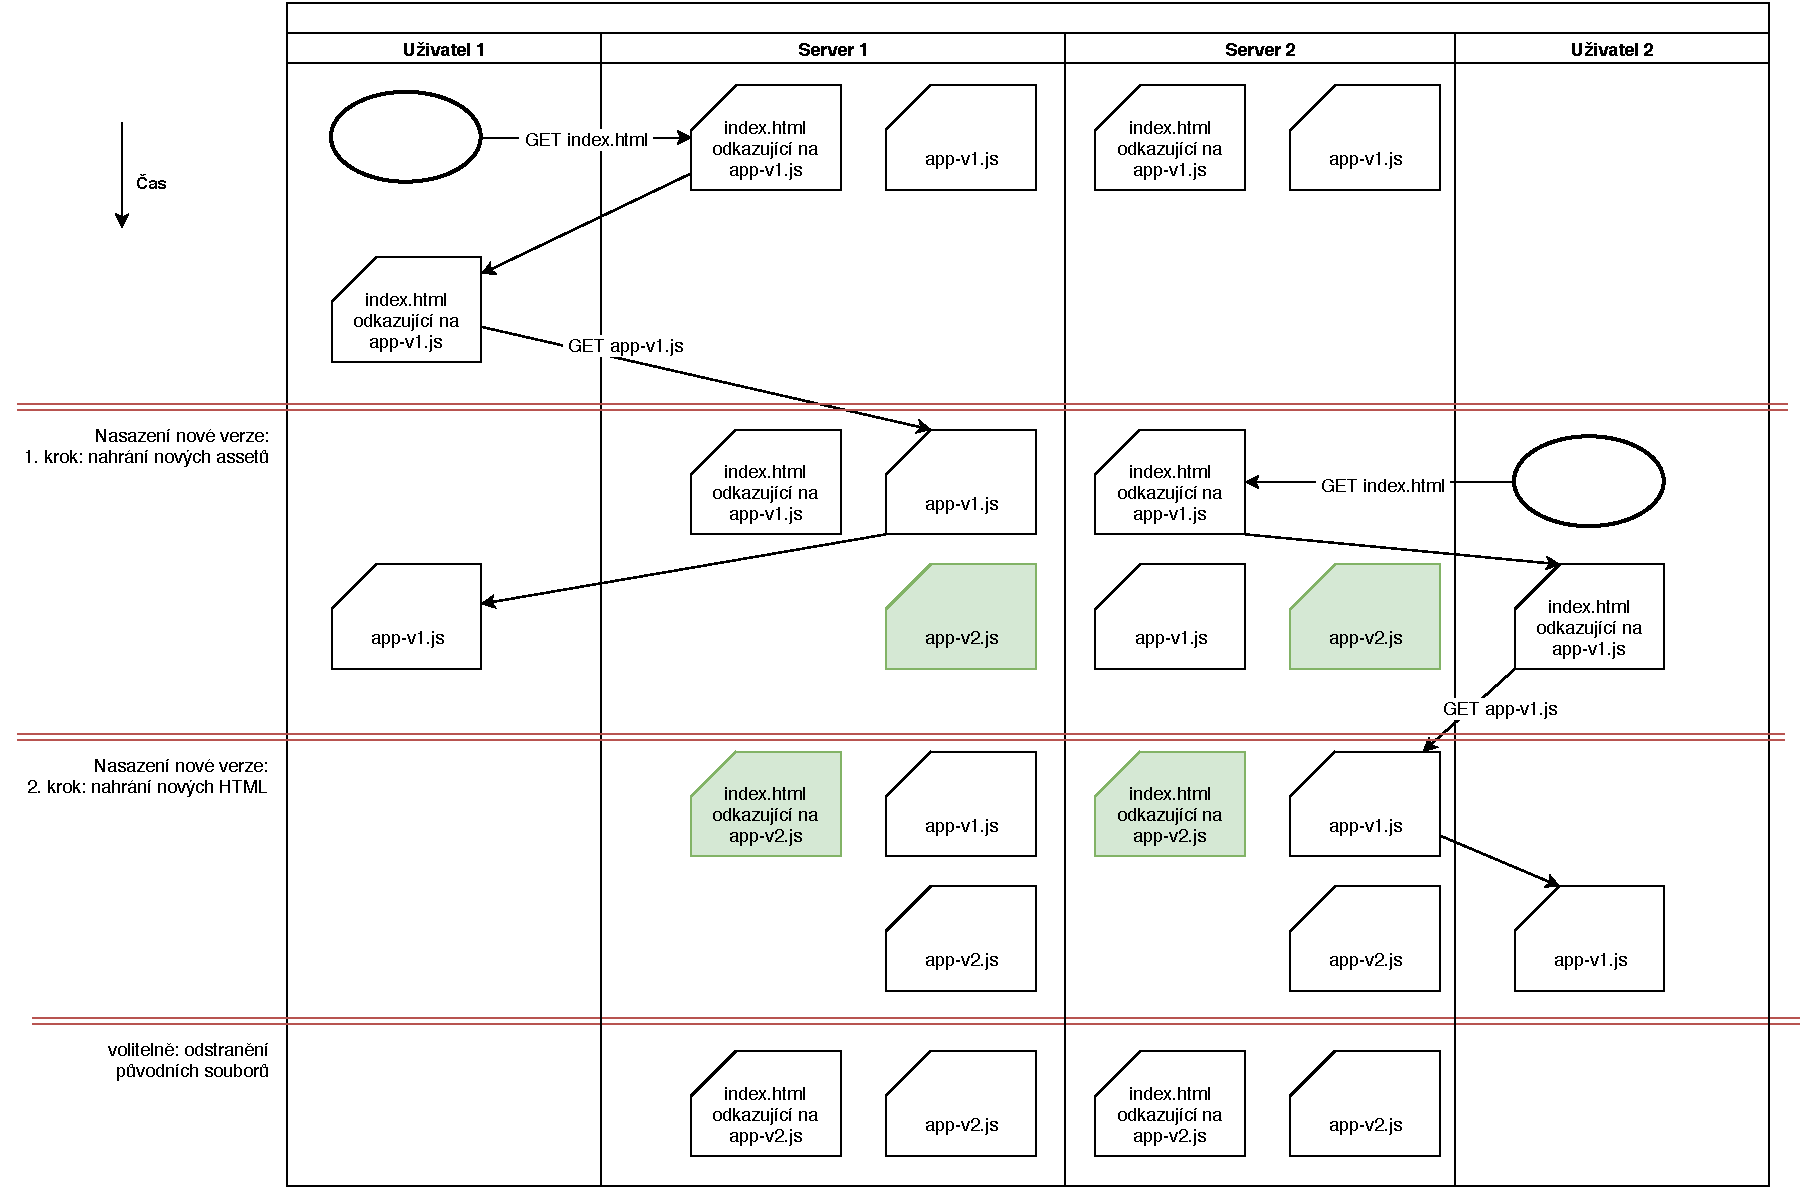
\includegraphics[width=1.2\textwidth]{media/static-deploy-changes.pdf}
            }
            \caption{Časový diagram znázorňující požadavky od dvou různých uživatelů ve dvou fázích nasazení nové verze statické aplikace. Uživatel 1 ilustruje nutnost nahrát nejprve na všechny servery sdílené assety. \HTML musíme nahrát až v druhé fázi, aby bylo garantované, že uživatelé co načtou novou verzi \HTML budou mít možnost ze všech serverů stáhnout odkazované zdroje. Uživatel 2 znázorňuje, proč je nutné uchovávat na serveru i starší verze zdrojů. Ty můžeme smazat až po nějaké delší době. Čas plyne odshora dolů, červené dvojité čáry reprezentují synchronizační bariéru.}
            \label{fig:static-deploy}
        \end{iffigure}

        Při použití kontejnerů nelze snadno dosáhnout toho, aby v containeru byly nové a současně staré zdroje. Místo toho se problém přesune na nějakou vyšší vrstvu, například ingress controller. Ten může podle \HTTP kódu odpovědi rozhodnout, jeslti se pokusí přeposlat požadavek na jiný kontejner. Pokud uživatel stáhne \HTML z nové verze aplikace, ale request na \glstext{CSS} přijde na starý container a vrátí kód \textit{404 Not Found}, může ingress controller GET požadavek přeposlat na nový kontejner, kde soubor existuje. Alternativou je použití session affinity, například pomocí cookies nebo \glstext{IP} adresy. Nebo lze mezi ingress controller a kontejnery umístit nějakou cachující \HTTP vrstvu (HAProxy, Varnish), která prakticky v základním nastavení načte a uloží do paměti zdroje z obou verzí. Je pouze nutné ošetřit, aby HTML ze starých kontejnerů nepřepsalo \HTML z kontejnerů nových, což může rozhodnout například podle hlavičky \code{Last-Modified-At}. Tento proces je vizualizován \pfxref{na diagramu}{fig:static-deploy-container}.

        \begin{iffigure}
            \centering
            \makebox[\textwidth][c]{
                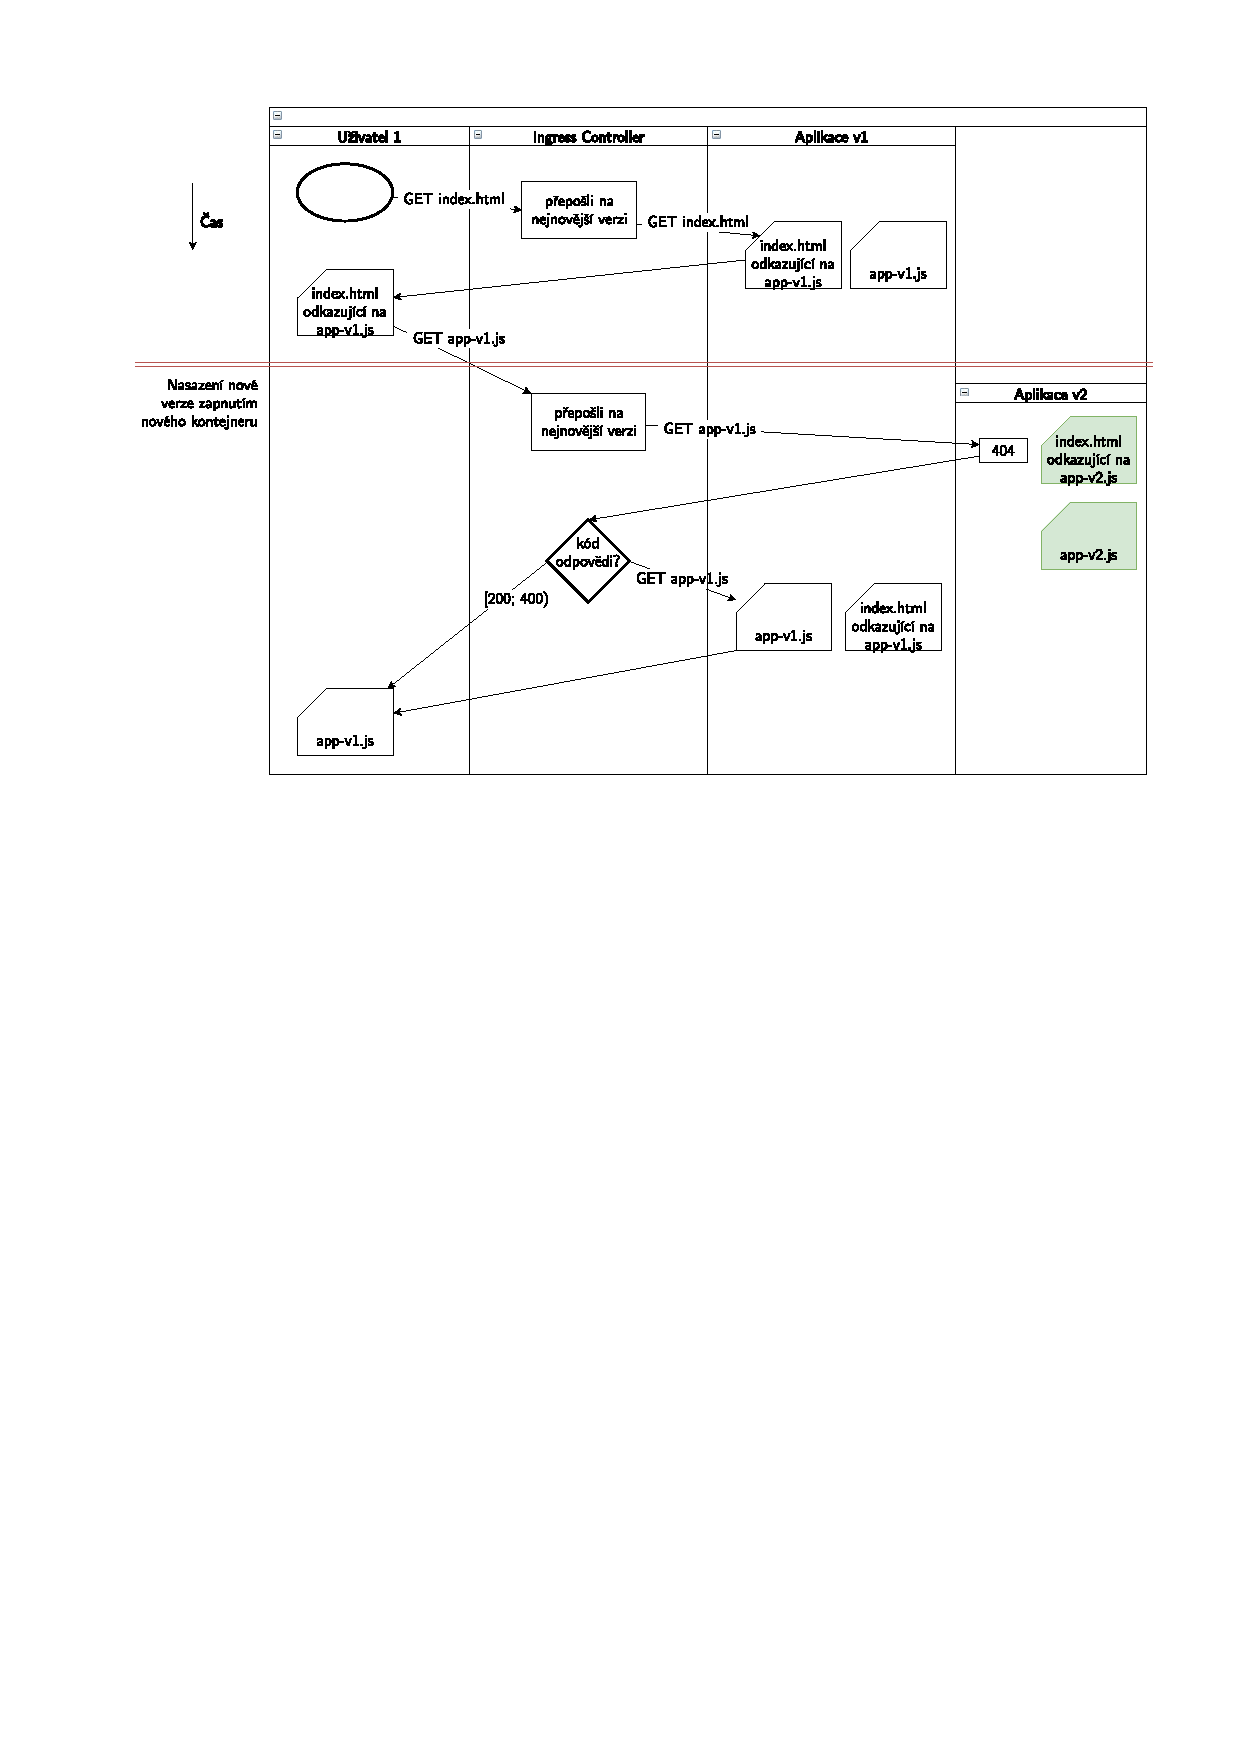
\includegraphics[width=1.2\textwidth]{media/static-deploy-kontejnery.pdf}
            }
            \caption{Časový diagram pro nasazení nové verze statické aplikace za použití kontejnerů. Pokud není praktické v nové verzi kontejneru uchovávat i starší verze zdrojů, je nutné implementovat nějakou komponentu (zde pojmenovanou \textit{ingress controller}), která při obdržení odpovědi s \glstext{HTTP} kódem 404 přepošle požadavek na starší verze aplikace. Toto chování je pro uživatele transparentní a projevuje se pouze lehce zvýšenou latencí.}
            \label{fig:static-deploy-container}
        \end{iffigure}

    \subsection{P2: Komplexní aplikace}
        V této kategorii uvažuji komplexní aplikace vyžadující relační databázi, případně další závislosti jako můžou být fronta, key-value storage, mailer, služba na zpracování obrázků nebo generování faktur, nebo platební brána. Na rozdíl od statických webů se tyto aplikace testují obtížně.
        U databáze například stačí spustit pro testy nový databázový stoj a spustit migrace. V případě platební brány která může od aplikace požadovat veřejně dostupnou url pro webhooks to může znamenat, že už samotný test vyžaduje nějakou úroveň nasazení aplikace.

        Pro testování jsem implementoval blog v PHP, konkrétně za použití frameworku Symfony \cite{symfony}. Aplikace při zpracování každého požadavku posílá dotazy na články do externí MySQL databáze. Dále komunikuje s key-value serverem Redis, kde spravuje session. Třetí závislost je API třetí strany: \code{mailgun.com}, které se používá pro posílání transakčních emailů.

    \subsection{P3: Aplikace distribuovaná jako kontejner}
        Aplikace v kontejneru mají stejné nároky na testovací prostředí jako aplikace v předchozí skupině a v rámci \CICD se liší pouze v buildu a nasazení. Jelikož samotné \CI často používá Docker, bude při tomto testu nutné řešit \glstext{DinD} nebo nějakou alternativu. Vystavěný Docker obraz je potřeba nahrát do nějakého repozitáře. Teoreticky lze obrazy exportovat/importovat i jako soubory, ale to není praktické, mj.~i proto, že se pak neuplatní sdílení jednotlivých vrstev obrazu. Některé systémy mají přímo zabudovaný registr obrazů a pro ostatní budu muset používat nějaký externí registr.


    \newpage
    \section{GitLab}
    GitLab je především systém pro správu repozitářů a vzniknul jako otevřená alternativa služby GitHub. Nabízí ale velmi kvalitní vlastní \CI a má nástroje podporující \CD. GitLab je poskytován jako \glstext{SaaS} a to jak v managed variantě, tak v placené self-hosted variantě. Existuje i fukčně velmi ořezaná self-hosted verze zdarma. Veřejné jádro je poskytované jako \textit{GitLab Community Edition}, placené části jsou vedeny jako \textit{GitLab Enterprise Edition}.

    Oficiálně GitLab podporuje celou řadu instalačních možností od balíčků pro klasické Linux distribuce, přes Docker kontejnery až po složitější šablony pro Kubernetes nebo OpenShift. Do podzimu 2018 byl GitLab distribuován jako monolitická aplikace, které se velmi obtížně škálovala a spouštěla distribuovaně v několika replikách. Podařilo se ale GitLab rozdělit na jednotlivé komponenty (gitaly: git repozitáře, gitlab-shell: HA api nad gitaly, mailroom: správa příchozích emailů, sidekiq, task-runner, unicorn: ruby webserver). Dále ma GitLab řadu externích závislostí: relační databázi (konkrétně PostgreSQL, podpora pro MySQL už neexistuje), key-value storage (Redis), úložitě pro objekty (AWS S3 nebo otevřená alternativa s kompatibilním api Minio). V oficiálním docker image, kterému říkají \textit{omnibus}, jsou všechny tyto závislosti přibalené. Nově vznikly separátní docker image pro každou GitLab službu zvlášť a šablony pro Kubernetes Helm, usnadnující jejich spuštění a konfiguraci.

    Protože jsou oba přístupy diametrálně odlišné, rozhodl jsem se nasadit GitLab jak v původním \textit{omnibus} variantě distribuované jako balíček pro Debian, tak ve variantě mikroslužeb v prostředí kontejnerů a porovnat obě varianty.

    \subsection{GitLab Omnibus}
        Instalace podle oficiální dokumentace je velmi jednoduchá. Jde jenom o přidání vlastního repozitáře a instalace balíčku~\cite{gitlab-install-ubuntu}. Po instalaci je rovnou spuštěna celá aplikace a při přístupu na HTTP endpoint se rovnou zobrazuje dialog pro nastavení administrátorského hesla.

        Aplikaci lze konfigurovat na několika místech: z webového rozhraní, \code{gitlab.yml} a \code{gitlab.rb}). V každé části je bohužel trochu něco jiného. V rámci této práce jsem upravil konfiguraci v \code{gitlab.rb}, kde jsem nastavil externí \glstext{URL}, na kterou GitLab generuje externí linky (například v emailové komunikaci), počáteční heslo pro administrátora a především token, kterým se bude autentifikovat GitLab Runner obstarávající \CI.

    \subsection{GitLab mikroslužby}
        GitLab začal oficiálně na konci roku 2018 podporovat také nasazení do Kubernetes přes Helm~\cite{gitlab-helm-chart}. Kubernetes je distribuovaný orchestrátor kontejnerů a Helm je balíčkovací aplikace. Každá komponenta GitLabu byla oddělena do samostatného docker obrazu a v Helm balíčku (\textit{Helm chart}) je pomocí Kubernetes zdrojů popsáno jak se dané kontejnery mají spouštět a jak jsou provázané. Teoreticky je možné kontejnery spouštět i ručně v jiném systému než Kubernetes, ale není to oficiálně podporované a neexistuje k tomu dokumentace.

        \begin{iffigure}
            \centering
            \makebox[\textwidth][c]{
                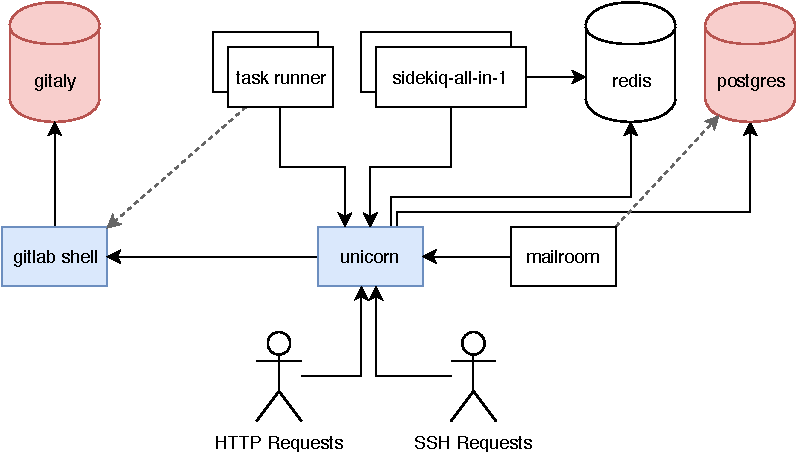
\includegraphics[width=1.0\textwidth]{media/gitlab-arch.pdf}
            }
            \caption{Architektura GitLab mikroslužeb a jejich propojení. Modře zvýrazněné komponenty jsou bezstavové, můžou běžet ve víc replikách a je před nimi nějaký load balancer. Zdvojené komponenty jsou workery a lze je horizontálně škálovat. Červeně jsou znázorněny \glstext{SPoF}, komponenty které ukládají stav a nelze je snadno distribuovat.}
            \label{pic:gitlab-architecture}
        \end{iffigure}

        Hlavní výhody nasazení GitLabu přes mikroslužby jsou:
        \begin{itemize}
            \item Přehlednost. Administrátor přesně ví, jaké komponenty systém obsahuje. Jednotlivé části nejsou skryté v Omnibus balíčku, kde se těžko dohledávají logy.
            \item Metriky mohou přímo využívat exportery nasazené v clusteru. V Omnibus jsou k dispozici pouze metriky pro celý balík, nebo je musí další proces uvnitř exportovat. To je další komplexita a nekonzistence se zbytkem prostředí.
            \item Lepší škálovatelnost. Můžeme škálovat pouze některé komponenty. Navíc díky přesným metrikám můžeme škálovat vytížené komponenty dynamicky.
            \item Využití upstream služeb. Řada komponent, které GitLab využívá, jsou nezměněné aplikace třetích stran. To je například ElasticSearch, Redis a relační databáze. V Omnibus balíčku jsou přibalené; nelze je aktualizovat a pokud na to GitLab nemyslel, nelze je vyčlenit a použít externí službu. U mikroslužeb má administrátor plnou kontrolu nad tím, které služby nasadí a pro které například použije cloudovou managed variantu.
        \end{itemize}

        Instalace GitLabu jako mikroslužeb je oproti verzi Omnibus velmi komplikovaná. Vyžaduje minimálně uživatelskou znalost Kubernetes a velmi podrobnou znalost Helm. Dokumentace je zatím (k lednu 2019) nekompletní a hodně nastavení a jejich význam je nutné dohledávat v šablonách Helm chartu. Některé konfigurace nejsou podporovánu vůbec. Narazil jsem například na nutnost nakonfigurovat Redis clusteru s heslem~\cite{gitlab-helm-issue-redis}. Například managed varianta od \glstext{AWS} podporuje přihlášení heslem pouze při použití \glstext{TLS} tunelu, protože bez něj se posílá heslo v plaintextu a nedává moc smysl vůbec heslo použít. To souvisí s tím, že GitLab mikroslužby jsou velmi nové; dá se očekávat, že čím víc firem bude takto GitLab nasazovat, tím lepší dokumentace a podpora pro různá prostředí vznikne.

    \subsection{GitLab \CI}
        \CI není přímo komponenta distribuovaná s GitLab, je ale dobře zaintegrovaná. Díky skvělému návrhu GitLab pouze vystavuje události na \glstext{API}. K API se může registrovat libovolné množství runnerů, které se periodicky \glstext{API} dotazují na nové práce ke spuštění~\cite{gitlab-runner-registration}. Runner může běžet na stejném serveru jako GitLab, ale velkou výhodou je možnost spustit runner i na jiném vzdáleném serveru -- například pro mobilní aplikace se často používá Mac mini s macOS, které je pro kompilaci nezbytné. Při registraci runneru je možné ho přidělit pouze některým projektům podle tagu, nebo ho zveřejnit pro všechny projekty.

        Runner při získání práce z \glstext{API} má k dispozici soubor s definicí (obsah souboru \code{.gitlab-ci.yml}~\cite{gitlab-runner-yaml}) a přístupové údaje k repozitáři. Architektura GitLab \CI se skládá z tzv. \textit{stages} (etapy) a \textit{jobs} (kusy práce), jak ilustruje \pfxref{diagram}{pic:gitlab-ci-architecture}. Jeden push do repozitáře typicky vygeneruje jednu \textit{pipeline}, což je sada \textit{stages} a \textit{jobs} popsaná konfigurací \CI v daném commitu.

        \begin{iffigure}
            \centering
            \makebox[\textwidth][c]{
                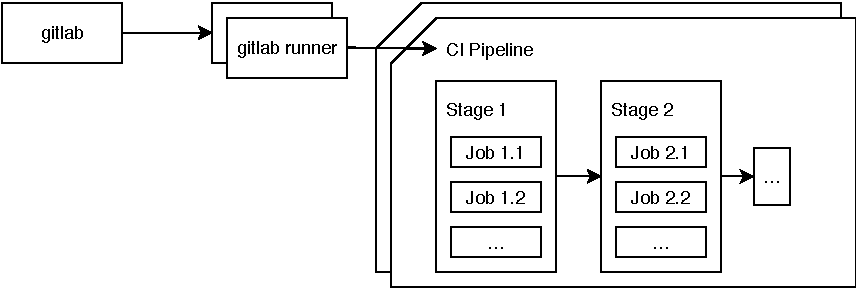
\includegraphics[width=1.0\textwidth]{media/gitlab-arch-ci.pdf}
            }
            \caption{Architektura GitLab CI. Runnerů i pipeline může existovat mnoho. V rámci jedné \textit{pipeline} je několik \textit{stages}, uvnitř kterých je sada paralelně spuštěných \textit{jobs}.}
            \label{pic:gitlab-ci-architecture}
        \end{iffigure}

        V konfiguračním souboru lze nastavit celou řadu pokročilejších funkcí~\cite{gitlab-runner-yaml}. Lze spouštět joby pouze pro určité kontexty podle kombinace proměnných prostředí a informace z verzovacího systému. Dále je možné joby provazovat podle závislostí a tím je serializovat. Toto ale není implementováno dokonale a všechny joby v rámci jedné stage běží najednou a čekají na doběhnutí všech jobů v předchozí stage. Celá pipeline tak může trvat delší dobu než je nutné.

        \label{gitlab-executor}
        V oficiální implementaci nabízí runner celou řadu možností, jak jednotlivé \textit{jobs} spouštět, tzv. \textit{executors}~\cite{gitlab-runner-config}. Základní je \code{shell}, při kterém neexistuje prakticky žádná izolace procesů a čištění prostředí. Jakékoliv závislosti, které je potřeba instalovat do sytému, ovlivňují všechny ostatní procesy na stejném serveru. Procesy běží pod neprivilegovaným uživatelem \code{gitlab-runner}, takže je lepší potřebné závislosti nainstalovat předem administrátorem. Tento executor může být vhodný pro dedikované prostředí pokud zajistíme, že tento server využívá pouze jeden projekt, případně pouze důvěryhodné nekolidující projekty. Velmi podobně funguje executor \code{ssh}, který místo na lokálním stroji spouští příkazy vzdáleně. Na cílovém stroji nejsou potřeba žádné závislosti (samozřejmě s výjimkou ssh serveru); v cloudovém prostředí může být praktické mít čisté virtuální stroje, na které se pak ssh runner připojuje. Dále lze ssh executor využít pro systémy, na kterých runner nemůže běžet lokálně. Velkou nevýhodou tohoto prostředí je nízká opakovatelnost. Jelikož se všechny joby mohou navzájem ovlivňovat a hostující systém se průběžně mění, při opakovaném spuštění nemusí starší joby už fungovat, přestože dřív procházely úspěšně. Ostatní executory tento problém do značné míry eliminují.

        Zbylé executory mají kompletní izolaci všech jobů. Možnosti \code{parallels} a \code{virtualbox} startují pro každý job nový virtuální stroj, z jednoho obrazu podle konfigurace runneru. Kontejnerizace jobů je nabízena v executoru \code{docker}: pro každý job je možné zvolit vlastní image. Varianta \code{kubernetes} je pro runner běžící v Kubernetes clusteru a vytváří pro každý job nový pod. Všechny tyto executory mají dobře opakovatelné joby. Pokud nezměníme obraz virtuálního stroje, případně pokud používáme stále stejný docker image, budou až na případné externí závislosti joby spuštěné identicky jako dřív.

        \label{sec:gitlab-ci-docker}
        Nastavení \CI se dále komplikuje při buildu Docker obrazů. Při použití většiny executorů máme dvě možnosti. První varianta je použít hostitelský Docker. U \code{shell} (a potažmo \code{ssh}) executoru stačí vyřešit oprávnění (typicky je potřeba přidat uživatele \code{gitlab-runner} do skupiny \code{docker}). U \code{docker} případně \code{kubernetes} executoru můžeme mountnout ovládací Unix socket \code{/var/run/docker.sock} do našeho kontejneru. Pro virtuální stroje by teoreticky šel socket mountnout také, ale když přijdeme o izolaci nemusíme pak \glstext{VM} používat vůbec. Nevýhodou tohoto řešení je, že všechny aplikace využívající \CI vidí obrazy a cache ostatních aplikací. Pokud se jedna z aplikací přihlásí do vzdáleného registru a stáhne nějaký soukromý obraz (\code{docker pull}), všechny ostatní aplikace tento obraz pak vidí a mohou ho číst i přesto, že nemají k vzdálenému registru oprávnění. Podobně jako při použití \code{shell} executoru tak musíme při sdílení Docker daemonu na \CI stavět pouze důvěryhodné aplikace.

        Druhou variantou buildu Docker obrazů je tzv. \textit{Docker in Docker} (\glstext{DinD}). To je Docker démon zabalený do Docker kontejneru. Při spuštění stále sdílí Linuxové jádro s hostitelským systémem, ale samotný Docker proces je izolovaný: má samostatný seznam procesů, vlastní limity a oddělenou build cache. \glstext{DinD} může být spuštěný právě pro jeden job. Ukázková specifikace pipeline pro Docker v kontejnerovém prostředí je popsána \pfxref{v kódu}{fig:gitlab-dind}.

        \begin{iffigure}
            \begin{minted}[frame=lines,framesep=2mm,linenos]{ruby}
services:
  - "docker:dind"

variables:
  DOCKER_HOST: "tcp://docker:2375"

build:
  stage: build
  script:
    - docker build --tag demo-build .
            \end{minted}
            \caption{Ukázkový soubor \code{.gitlab-ci.yml} pro nastavení \glstext{DinD}.}
            \label{fig:gitlab-dind}
        \end{iffigure}

        Při samostatně spuštěném \glstext{DinD} pro každý build máme perfektní izolaci všech klientů, ale přicházíme o některé výhody Dockeru, konkrétně o stažené obrazy a cache předchozích buildů. To je známý problém a GitLab ho bez úspěchu řeší už několik let~\cite{gitlab-docker-artifact-caching}. Největší výhoda tohoto řešení je perfektní dostupnost: každá pipeline má vlastní Docker a případné aktualizace se dějí na úrovni změny obrazu v \code{.gitlab-ci.yml}. Přes GitLab mechanizmus pro cachování lze uložit Docker data a při dalším jobu je opět nahrát do nového Docker daemona~\cite{patel-docker-cache}. Toto řešení je ale velmi pomalé. Obrazy včetně cache budou běžně kolem stovek megabajtů a zapisujeme je dokonce hned čtyřikrát: jednou na disk při exportu, potom do GitLab cache což je často externí objektové úložiště (jako je AWS S3) a po čtvrté při načítání do prázdného Dockeru. Pro aplikace s extrémně dlouhým buildem v řádu desítek minut to může být přínosné, ale pro typické webové aplikace na které se tato práce soustředí není toto řešení vhodné.

        Velmi úspěšně lze ale \glstext{DinD} provozovat jako dlouhožijící službu oddělenou od samotné \CI pipeline. Získáme tím tak výhody obou řešení a veskrze eliminujeme všechny nevýhody. Pro každou skupinu navzájem si věřících aplikací spustíme samostatný \glstext{DinD} proces. Ten může běžet na hostitelském serveru s \CI nebo libovolném externím. V daných pipeline specifikacích pak stačí neuvést \code{services: "docker:dind"} a nakonfigurovat proměnnou \code{DOCKER\_HOST} (například \code{tcp://group-7.external-docker.local:2375}). Každá skupina aplikací uvidí pouze svoje obrazy a bude mít persistentní cache. Nevýhodou tohoto řešení je vysoká komplexita. Je nutné nějakým způsobem zajistit, aby se k Docker socketu mohly připojit pouze autorizované aplikace. Na to je praktické použít nějakou pokročilou abstrakci, například Network Policies v Kubernetes. Samotná \glstext{ACL} logika může být v síťové vrstvě jako je například Weave, Contrail nebo Calico, nebo v samostatném dedikovaném firewallu.

    \subsection{Podpora \CD praktik}
        Ve svém marketingovém copy se GitLab prezentuje jako jednotný systém pro \CICD, monitoring a bezpečnost. Jak jsem popsal v předchozí sekci, \CI nabízí GitLab perfektní. Co se týče podpory \CD, funkce GitLabu jsou omezené:

        \textbf{Environments} přináší přehled všech prostředí (například beta, produkce, \ldots) a nasazení do těch to prostředí~\cite{gitlab-environments}. Užitečná je možnost spouštět z tohoto zobrazení deploy znovu. Lze spustit i deploy nějaké starší verzi a udělat tak rollback. Při vhodném rozdělení pipeline na build a deploy je spuštění z tohoto přehledu je rychlejší, než spouštět celou pipeline. GitLab nenabízí žádnou možnost jak rollback omezit a je pouze na uživatelích, aby nespustili rollback na nějakou starou nekompatibilní verzi.
        \textbf{Review Apps} jsou prodávány jako systém, díky kterému lze nasadit zkušební verze aplikace do oddělených dynamických prostředí~\cite{gitlab-review-apps}. Prakticky to jde udělat v libovolném \CI systému; pro vybrané větve se spustí deploy a dynamicky se předá nějaký identifikátor pro veřejnou \glstext{URL} a další konfiguraci, to může být například název dané větve. Jediné co přináší GitLab je podpora pro dynamické \textit{Environments} bez nutnosti programovat to přes \glstext{API}, a tlačítko \textit{Stop} v webovém rozhraní, které spustí pipeline job která má na starost job vypnout. Veškerá praktická implementace je ale na vývojáři: GitLab neřeší nasazení a vypnutí aplikace, pouze zavolá uživatelem definovaný job.
        \textbf{Auto DevOps}~\cite{gitlab-auto-devops}. Tato kontroverzní~\cite{gitlab-auto-devops-forum} funkce GitLabu je zjednodušeně řečeno jenom hodně komplikovaný \code{.gitlab-ci.yml} soubor, který uživatel nevidí a použije se, pokud není v repozitáři jiná konfigurace pipeline. Auto DevOps pipeline má kolem 1000 řádek a obsahuje pokročilé Yaml konstrukce jako jsou reference a vnořování, které zhoršují čitelnost. Navíc do toho míchají bash scripty a využívají docker kontejnerů. Celá pipeline je ve výsledku hodně složitá. Auto DevOps podporuje pouze nasazování do Kubernetes clusteru. Build aplikace funguje jenom když je aplikace samotná stavěná pomocí \code{Dockerfile}. Distribuce obrazu musí být pomocí GitLab Container Registry. Deploy probíhá pomocí Helm. Lze použít výchozí Helm Chart distribuovaný s Auto DevOps, nebo použít vlastní. Ve vlastním Helm Chartu, resp. v konkrétních Kubernetes zdrojích, lze pak ručně nakonfigurovat vlastnosti rolling-update konkrétní aplikace a obecně škálování a dostupnost. Ve výchozím nastavení není explicitně rolling-update nakonfigurován.

        Ze všech systémů které řeší \CI a zároveň \CD je GitLab se svým Auto DevOps nejdál. Je ale velmi dogmatický a nebude fungovat s žádnou odchylkou v infrastruktuře.

        Drobnější funkce GitLabu podporující \CD:
        \begin{itemize}
            \item Možnost spouštět vybrané joby v pipeline pouze manuálně. Jedno z možných použití je deploy aplikace z \code{master} větve, kde vývojář může ručně spustit job pro deploy po doběhnutí předchozích automatických jobů. Bohužel všechny automatické joby definované v následujících stages se spouští bez čekání na manuální job a to i tehdy, když mají definované závislosti na manuálním jobu~\cite{gitlab-issue-manual-job}.
            \item Plánované spuštění pipeline. Přestože lze build spouštět programaticky z \glstext{API} z libovolného cronu, je užitečné že to má GitLab přímo implementované. Typické použití je tzv.~\textit{nightly build}.
            \item \textbf{Web terminals} umožňují připojit se do aplikačního kontejneru v Kubernetes clusteru. Podobně jako u Auto DevOps je tato integrace dogmatická a nekompatibilní s klasickým použitím Kubernetes labels~\cite{gitlab-issue-k8s-deploy}.
        \end{itemize}

    \subsection{Open-source}
        GitLab je vyvíjen jako otevřený software, v tom smyslu, že veškerý kód je veřejně čitelný. Některé části jsou opravdu open-source i co se licence týče: GitLab \glstext{CE} je pod \glstext{MIT} licencí. Jiné části, například GitLab \glstext{EE}, jsou pod vlastní licencí. Licence dokonce ani nedovoluje \glstext{EE} verzi provozovat bez zakoupené licence.

        Příspěvky a návrhy na změny kódu od lidí mimo GitLab Inc. jsou možne, ale vesměs ignorované. Jako přispěvatel jsem hodně cítil, že firma GitLab je čistě remote a nemá žádné kanceláře a tým na jednom místě~\cite{gitlab-team}. Většina návrhů na změnu -- od jednořádkových oprav po drobnější funkční úpravy -- co jsem poslal zůstala bez povšimnutí. To je tím spíš mrzuté, když razí cestu „minimum konfigurace, radši pošlete návrh na úpravu kódu pro všechny“~\cite{gitlab-no-custom}.

        U jednoho úkolu do kterého jsem se víc zapojil trvalo rok a půl začlenit drobnou změnu. Na tyto změny čekalo několik desítek firem. Šest vývojářů poslalo nezávisle na sobě návrhy na změnu. Změny byly vesměs triviální, bez dopadu na ostatní části kódu, byly otestované a dobře zdokumentované. Po opakovaném urgováním přes oficiální kanál podpory se u úkolu vyjádřil zaměstnanec GitLab. Bohužel se pouze zeptal, kdo má tuto část kódu na starost a tím na dva měsíce úkol opět usnul. Když se po dalším urgování přes podporu úkolu někdo chopil, zadání vesměs nepochopil a snažil se protlačit nepoužitelné řešení. Nechal si naštěstí problém znovu vysvětlit a řešení přehodnotil. Nakonec byl celý problém vyřešen a změny jsou zařazeny do vydání 11.8, tedy skoro 2 roky po otevření úkolu. Celé vlákno je veřejně na GitLab Issue Trackeru~\cite{gitlab-issue-slow}. Podobnou zkušenost mám i z několika dalších GitLab projektů, včetně aktivně vyvíjeného GitLab Helm Chart.

    \subsection{Rozšiřitelnost}
        Primární bod pro integraci s GitLabem jsou webhooky, které jsou vyvolané v reakci na systémové nebo projektové události~\cite{gitlab-webhooks}. Alternativou jsou tzv.~pluginy, což jsou spustitelné soubory na disku aplikačního serveru, které přijímají identický vstup a události jako webhooky ~\cite{gitlab-plugins}. Obě varianty jsou pouhé informace pro externí aplikace a neumožňují nijak rozšiřovat zabudované funkce nebo \glstext{UI} GitLabu.

    \subsection{Zálohování}
        GitLab nabízí nástroj, který zálohuje všechny komponenty: databázi, objektová úložiště (přílohy, výsledky \CICD, Docker Registry, Git \glstext{LFS}) a Git repozitáře. V Omnibus balíčku bez externích komponent je tedy zálohování snadné. Při rozdělení na mikroslužby se zodpovědnost za zálohování částečně přesouvá: u databáze a objektového úložiště (např.~\textit{AWS S3}) typicky na poskytovatele cloud řešení.

        Záloha kterou GitLab vytváří není atomická. Databáze se sice zálohuje v jedné transakci, ale ostatní komponenty žádné snapshoty obecně nepodporují. To lze simulovat vypnutím aplikace a vytvořením záloh. Nicméně, díky tomu že GitLab nejprve zálohuje databázi a potom ostatní data, nejpravděpodobněji se stane to, že ve výsledném balíčku budou nahrána i data na která nic neodkazuje. Nemůže se např.~stát, že by komentář obsahoval neexistující obrázek.

    \subsection{Zabezpečení}
        Podle \glstext{CVE} Details měl GitLab nejvíc kritické problémy -- hodnocené podle podle \glstext{CVSS} -- zjištěné v posledním roce (2018)~\cite{cve-gitlab}. To může souviset s exponenciálním růstem, který zažili díky \code{\#movingtogitlab} a akvicizi konkureční firmy GitHub firmou Microsoft~\cite{gitlab-growth}. Není zatím jasné, jestli dramatický nárůst počtu uživatelů přilákal bezpečnostní analytiky, nebo jestli bezpečnostní problémy jsou výsledkem zrychleného vývoje a zhoršení kvality produktu.

        %\todo{Jak dlouho trvá gitlabu opravit cve a zverejnit security fix?}

        Správa problémů (\textit{issues}) u projektů na GitLabu má možnost vytvořit nový záznam v důvěrném režimu. Takové problémy jsou pak viditelné pouze pro správce repozitáře. To je vhodné pro \textit{responsible disclosure} (zodpovědné zveřejnění) bezpečnostních chyb. GitLab toto úspěšně používá i pro vlastní projekty.

        GitLab zavádí v kontextu \CICD nový pojem \textit{continuous security testing} (kontinuální bezpečnostní testování)~\cite{gitlab-app-security}. Na rozdíl od testování po začlenění změn a nasazení, GitLab umožňuje každému vývojáři deploynout danou větev verzovacího systému do vlastního testovacího prostředí. To je znázorněno \pfxref{v diagramu}{fig:gitlab-review-cycle}.

        \begin{iffigure}
            \centering
            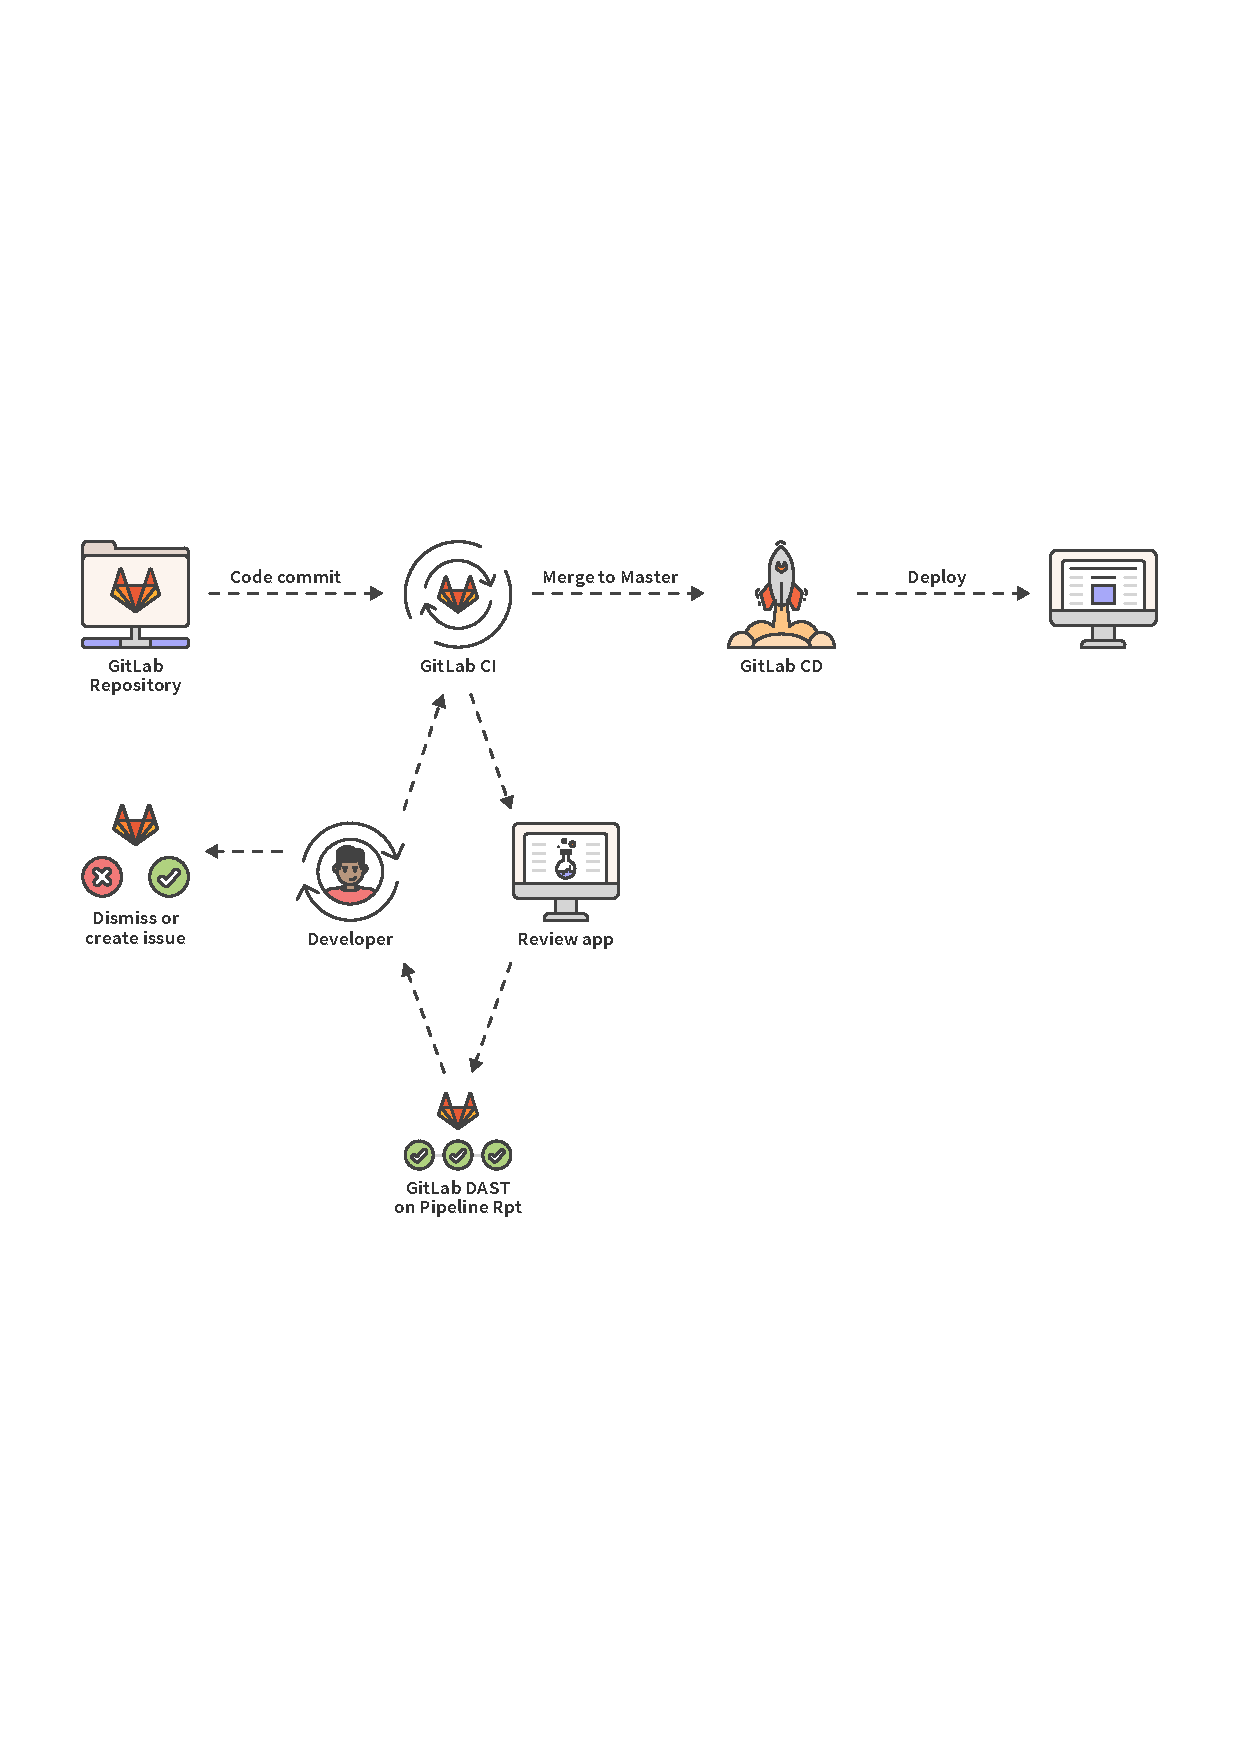
\includegraphics[width=\textwidth]{media/gitlab-review-cycle.pdf}
            \caption{Cyklus kontroly kvality aplikace GitLab s integrovaným \glstext{DAST}~\cite{gitlab-app-security}. Vývojář může vyhodnotit bezpečnostní problémy před začleněním změň do sdíleného kódu.}
            \label{fig:gitlab-review-cycle}
        \end{iffigure}

    \subsection{Dostupnost}
        S GitLabem mám praktické zkušenosti a provozuji ho pro přibližně 50 lidí. Zhruba 5 měsíců jsem používal balíček \textit{Omnibus} a s GitLab mikroslužbami pracuji podobně dlouho. Vyzkoušel jsem si i migraci z Omnibus na mikroslužby.

        Obě varianty nasazení byly při běžném používání (tzn. ne při správě) dobře dostupné. Většina výpadků nastala při problematických datech, které měly za následek extrémní zpomalení z pohledu uživatele. Jeden uživatel například nahrál $300$~MiB dump databáze a GitLab, resp. Gitaly, začal při počítání \textit{diff} padat. Jeden projekt tak omezil všechny ostatní projekty. GitLab by mohl mít nastavené lepší limity aby těmto výpadkům předešel, ideálně dynamicky podle dostupných zdrojů.

        \subsubsection{GitLab omnibus}
            Omnibus distribuce GitLabu, tedy balíček který obsahuje všechny komponenty, je primárně pro snadné nasazení a nepočítá se s tím, že by běžel s vysokou dostupností (\HA). Umožňují ale aktualizovat systém bez výpadku: doporučený postup je aktualizovat balíček, spustit databázové migrace a reloadnout webový frontend a konzumenty fronty~\cite{gitlab-omnibus-update}. Důsledně se snaží dodržovat kompatibilitu napříč verzemi a databázové migrace dělají zpětně kompatibilní. V každém vydání nové verze jsou změny rozepsané a případné nekompatibility jsou znázorněny v tzv. \textit{upgrade barometer}.

            V základním nastavení nelze GitLab Omnibus replikovat. Některé komponenty lze ale vyčlenit. Nezbytné jsou PostgreSQL a Redis. Jediné co pak zbývá a sdílí se mezi replikami jsou samotné git repozitáře na souborovém úložišti. Vyzkoušel jsem, že GitLab Omnibus správně funguje ve víc replikách, když se vyčlení databáze a repozitáře se sdílí přes \glstext{NFS}. Jedná se ale o nezdokumentované nasazení a nemá oficiální podporu.

            Při nasazení ve víc replikách lze docílit 100 \% dostupnosti při aktualizaci na novější verzi.

        \subsection{GitLab microservices}
            \pfxref{Na diagramu}{pic:gitlab-architecture} (strana~\pageref{pic:gitlab-architecture}) je znázorněna architektura GitLab mikroslužeb. Mikroslužby jsou obecně vhodné pro \glstext{HA} systémy:

            \begin{quote}
                [\ldots] each microservice in microservice architectures is operationally independent from others, and the only form of communication between services is through their published interfaces. This is fundamental since this allows one to change, fix or upgrade a microservice without compromising the system correctness, provided that the interfaces are preserved. \textit{Dragoni et al.~\cite{dragoni-microservices}}
            \end{quote}

            Klíčové komponenty GitLabu můžeme provozovat ve víc replikách a aktualizaci dělat pomocí rolling update, naprosto transparentně pro ostatní části systému. Některé komponenty jako jsou konzumenti fronty a manažer příchozích emailů můžeme dokonce aktualizovat s krátkým výpadkem, bez pozorovatelného dopadu pro uživatele.

            Správa stavových služeb je v distribuovaném systému nejkomplikovanější. GitLab jich bohužel používá celou řadu: relační databázi PostgreSQL, key-value storage Redis a vlastní služby Gitaly pro správu repozitářů. PostgreSQL s master-slave architekturou lze provozovat s vysokou dostupností použitím hot standby instance~\cite{kim-postgres}. Redis také používá master-slave architekturu, ale dokáže si v případě výpadku sám zvolit v clusteru nový master díky komponentě Redis Sentinel~\cite{redis-ha}. Tyto služby poskytovatelé cloudu nabízí i se správou, kde zodpovídají za dostupnost a některé aktualizace.

            Služba Gitaly je v oficiálním Helm chartu \glstext{SPoF}. Vystavuje \glstext{gRPC} \glstext{API} nad git repozitáři, se kterým pracuje většina ostatních komponent. Gitaly běží v jedné replice a je závislé na stavových datech na disku. Konzultoval jsem tento problém s oficiální podporou a je možné Gitaly provozovat nad \glstext{NFS} ve více replikách. Jde o kompromis mezi dostupností a rychlostí. Gitaly je z části limitováno propustností disku a \glstext{NFS} některé operace zpomalí.

            V oficiální distribuci má GitLab \glstext{SPoF} v Gitaly a při aktualizaci této komponenty je nedostupný. Při použití mikroslužeb s Gitaly nad \glstext{NFS} je GitLab bez výpadku dostupný pro použití i pro správu a dostupnost lze zvyšovat přidáním dalších replik.

    \subsection{Integrace}
        GitLab~\CI vyžaduje repozitáře na GitLab. Kromě celé řady variant importu z různých externích úložišť (včetně GitHub, Bitbucket a desítky dalších) lze také vytvořit mirror libovolného repozitáře. Lze tak de facto použít GitLab~\CI s jakýmkoliv repozitářem.

        Integrace s externími službami má GitLab suverénně nejlepší ze všech testovaných systémů. V základu je zabudovaných přes 30 služeb, od chatovacích služeb po správy úkolů a některé ovlivňují i \glstext{UI}. Například \textit{External Wiki} přidává do panelu odkazů novou položku.

        GitLab má zabudovanou podporu pro nasazování do Kubernetes. Authentikace je možná pouze přes token a nelze využít například certifikáty nebo externí authentikační službu. Po počáteční instalaci komunikuje GitLab s Kubernetes přes balíčkovací systém Helm. Deploy do Kubernetes může fungovat bez další konfigurace díky Auto DevOps~\cite{gitlab-auto-devops}. Dokonce v základu fungují i Review Apps~\cite{gitlab-review-apps}.

    \subsection{Praktické nasazení projektů}
        \subsubsection{Projekt 1}
            \label{subsec:gitlab-p1}
            Nastavení pipeline pro statický projekt není vůbec přímočaré. Z webového rozhraní jsem vytvořil projekt včetně repozitáře, v lokálním git repozitáři jsem nastavil přidělený remote a zdrojové kódy jsem nahrál na GitLab. Potom jsem ručně napsal konfiguraci pipeline v souboru \code{.gitlab-ci.yml}. Protože jsem GitLab runner nasadil s executorem \code{shell}, nainstaloval jsem předem do sdíleného prostředí nezbytné závislosti. Popis instalace Ruby, Gem a balíčků Jekyll a Bundler jsem popsal \pfxref{v příloze}{ch:implementace}. Konfigurace GitLab pipeline obsahuje značné množství klíčových slov, ale má vynikající webovou dokumentaci. Uvítal jsem také podporu schématu v \glstext{IDE} IntelliJ IDEA~\cite{idea-gitlab-plugin}, bez kterého se těžko s JSON pracuje.

            Pipeline jsem specifikoval dvoukrokovou. V prvním kroku se generují výstupy a výsledky se archivují jako tzv.~artefakty. V kroku druhém  se tyto artefakty stáhnou a nahrají na webový server. Díky tomuto rozdělení lze na GitLabu deploy opakovat bez nutnosti znovu generovat všechny artefakty. To umožňuje mj.~velmi rychlý rollback a obecně přesun mezi verzemi.

            Implementoval jsem podporu pro GitLab review apps. Změny z větve \code{deploy/prod} se automaticky nahrávají do produkčního prostředí. Ostatní větve se nasadí pro dynamicky vygenerovaného prostředí a vývojář je má po kontrole možnost ručně vypnout.

            Při použití \code{docker} executoru je pipeline stejně jednoduchá, ale odpadá nutnost předem nastavit prostředí a není nutné řešit kolize závislostí napříč projekty. GitLab dokáže artifacts ukládat z kontejneru stejně jako v \code{shell} executoru.

        \subsubsection{Projekt 2}
            Pipeline pro dynamický komplexní projekt je překvapivě podobná, jako u statického projektu. Opět jsem vytvořil dvě hlavní stage: build a deploy. Hlavní rozdíl je v samotných příkazech pro sestavení, které jsem abstrahoval do \code{Makefile}. Protože využívám \code{shell} executor, předinstaloval jsem \glstext{PHP}, balíčkovací systém composer a další. To je bohužel správa kterou je potřeba dělat mimo konfiguraci pipeline.

            Review apps jsem navrhnul teoreticky, protože bez kontejnerů je implementace zbytečně složitá. U relační databáze (ve smyslu \glstext{RDBMS}) je potřeba vytvořit novou databázi, nakonfigurovat oprávnění pro nového uživatele aby nemohl ovlivnit ostatní (a hlavně produkční) databáze, nakonfigurovat aplikaci aby používala jiné databázové údaje a spustit migrace. Dále je potřeba po ukončení review app nějakým způsobem tuto databázi smazat. Velmi podobný postup je potřeba opakovat pro key-value storage, na které je aplikace také závislá.

        \subsubsection{Projekt 3}
            Opět jsem použil úplně stejnou pipeline jako pro předchozí dva projekty. Pro sdílení vystavěného docker obrazu jsem použil GitLab Container Registry, což je vestavěná služba. Registr je automaticky založený při vytvoření GitLab projektu. V build scriptu jsem provedl authentikaci \code{docker login}. Heslo jsem hardcodoval rovnou do scriptu. Alternativně může být nastaveno ve webovém rozhraní GitLabu a předáno do jobu jako proměnná prostředí (\code{env}). To má smysl hlavně pro veřejné projekty, kde nechceme heslo zveřejňovat; pak je ale nutné ohlídat, aby \CI job nemohl kdokoliv škodlivě upravit, spustit, a nechat si vypsat heslo do logu.

            Pro build aplikace se používá hostitelský docker démon. Celou řadu výhod a nevýhod a alternativní řešení jsem rozepsal \pfxref{v sekci o Dockeru}{sec:gitlab-ci-docker}.

            Pro spuštění aplikace na webovém serveru se nejprve nahraje soubor pro konfiguraci Docker Swarm stacku. Na webovém serveru se pak spustí přihlášení do registru a příkazem \code{docker stack deploy} se spustí a případně aktualizuje aplikace.

            U tohoto ukázkového projektu si použitím \code{docker} executoru moc nepomůžeme. Docker jako závislost musí být na hostitelském serveru předinstalovaný a pro zbytek se používají kontejnery.


    \newpage
    \section{Jenkins}
\label{sec:jenkins}
    Jenkins byl dřív známý jako Hudson a přejmenoval se po neshodě s Oracle \cite{jenkins-hudson}. Oba projekty pak nějakou dobu byly udržovány souběžně. Oracle svůj systém Hudson oficiálně nikdy nepřestal vyvíjet, ale poslední vydání je ze začátku roku 2016. V následujícím textu se budu věnovat pouze Jenkins, který je dodnes aktivně udržován a má velkou komunitu.

    Hlavní výsadou Jenkins oproti ostatním \CICD systémům je rozšiřitelnost pomocí pluginů.
    \todo{popsat ze jenkins je jenom o pluginech}\blind[1]

    Architektura Jenkins je master+agents \cite{jenkins-architecture}. Stavová master instance poskytuje \glstext{API} a webové \glstext{GUI} a koordinuje práci jednotlivých bezstavových agentů (workerů).

    \subsection{Instalace a konfigurace}
        Instalace Jenkins z oficiálního balíčku je přímočařá. Nejprve jsem zaregistroval Jenkins \glstext{APT} repozitář \code{pkg.jenkins.io} a aplikaci nainstaloval. Jenkins ale odmítal nastartovat, protože mu chyběl Java runtime. Očekával bych, že aplikační balíček bude mít nezbytné závislosti minimálně v \textit{suggested packages}. Jenkins v aktuální verzi podporuje pouze Java 8 \cite{jenkins-java}. To je \glstext{TLS} verze z března 2014, která má komerční podporu pouze do ledna 2019 \cite{oracle-eol}.

        Při prvním zobrazení webového rozhraní se provádí konfigurace a volitelná instalace rozšíření. Na rozdíl od např. GitLabu nebo Wordpressu vyžaduje Jenkins výchozí administrátorské heslo, které vygeneroval na disk.

        V roce 2018 přišel Jenkins s možností nahradit ruční klikání konfigurace ve webovém rozhraní kódem (\glstext{CasC}) \cite{jenkins-casc}. Některá klíčová nastavení, konkrétně třeba správa rozšíření, je zatím nestabilní. Dále je nahlášena celá řada nekompatibilit s různými rozšířeními \code{jenkins-casc-compat}.

        Každý projekt je na Jenkins nutné založit a nakonfigurovat ručně. Některá rozšíření tento problém řeší, například \code{GitHub Branch Source Plugin} \cite{jenkins-plugins-gbs} sleduje všechny repozitáře vybraných GitLab uživatelů a pokud v nich najde \code{Jenkinsfile}, založí pro repozitář nový projekt na Jenkins. Původně byly Jenkins projekty konfigurovatelné jenom z webového rozhraní a \glstext{API}. V roce 2014 byla publikován \code{Pipeline Plugin}, který umožňuje popsat konfiguraci projektu skriptem. Na to v roce 2016 navázalo rozšíření \code{Pipeline Model Definition Plugin}, které přináší podporu pro deklarativní popis pipeline, kde Jenkins říkáme co se má stát, ale ne nutně \textit{jak}. Deklarativní pipeline je doporučený způsob nastavení Jenkins projektů \cite{jenkins-best-practices}.

        Problém Jenkins je uživatelské rozhraní. Ve výchozím stavu má \glstext{UI} celou řadu velmi problematických částí: několika-úrovňové menu, které vyžaduje přesný pohyb myší; nesjednocené symboly, navíc často nekonvenční (například modrá koule u úspěšného jobu místo klasické zelené); konfigurace a všechny formuláře jsou složité a běžně obsahují 100+ vstupů. Rozšíření Blue Ocean nabízí alternativní \glstext{UI} pro zobrazení průběhu a výsledků buildů \cite{jenkins-plugin-blueocean}. Bohužel nemodernizuje zbytek Jenkins, administraci. Pokud uživatelé konfigurují projekty výhradně přes \code{Jenkinsfile}, nemusí do původního rozhraní vůbec přistupovat. Osobně mi rozhraní přišlo hezké, ale oproti konkurenčním \CICD pomalé.

    \subsection{Rozšiřitelnost}
        Jenkins má v oficiálním registru přes $1\,500$ rozšíření. Používaných je jich ale jenom zlomek; jak ukazuji \pfxref{na grafu}{fig:jenkins-plugins} často instalovaných rozšíření je jenom kolem $200$. Velmi překvapivé bylo zjištění, že rozšíření jsou často aktualizovaná. \pfxref{Z grafu}{fig:jenkins-plugins-update} lze vidět, že přes $600$ rozšíření mělo vydání v posledním roce.

        \afterpage{
            \begin{iffigure}
                \centering
                \begin{subfigure}[b]{\textwidth}
                    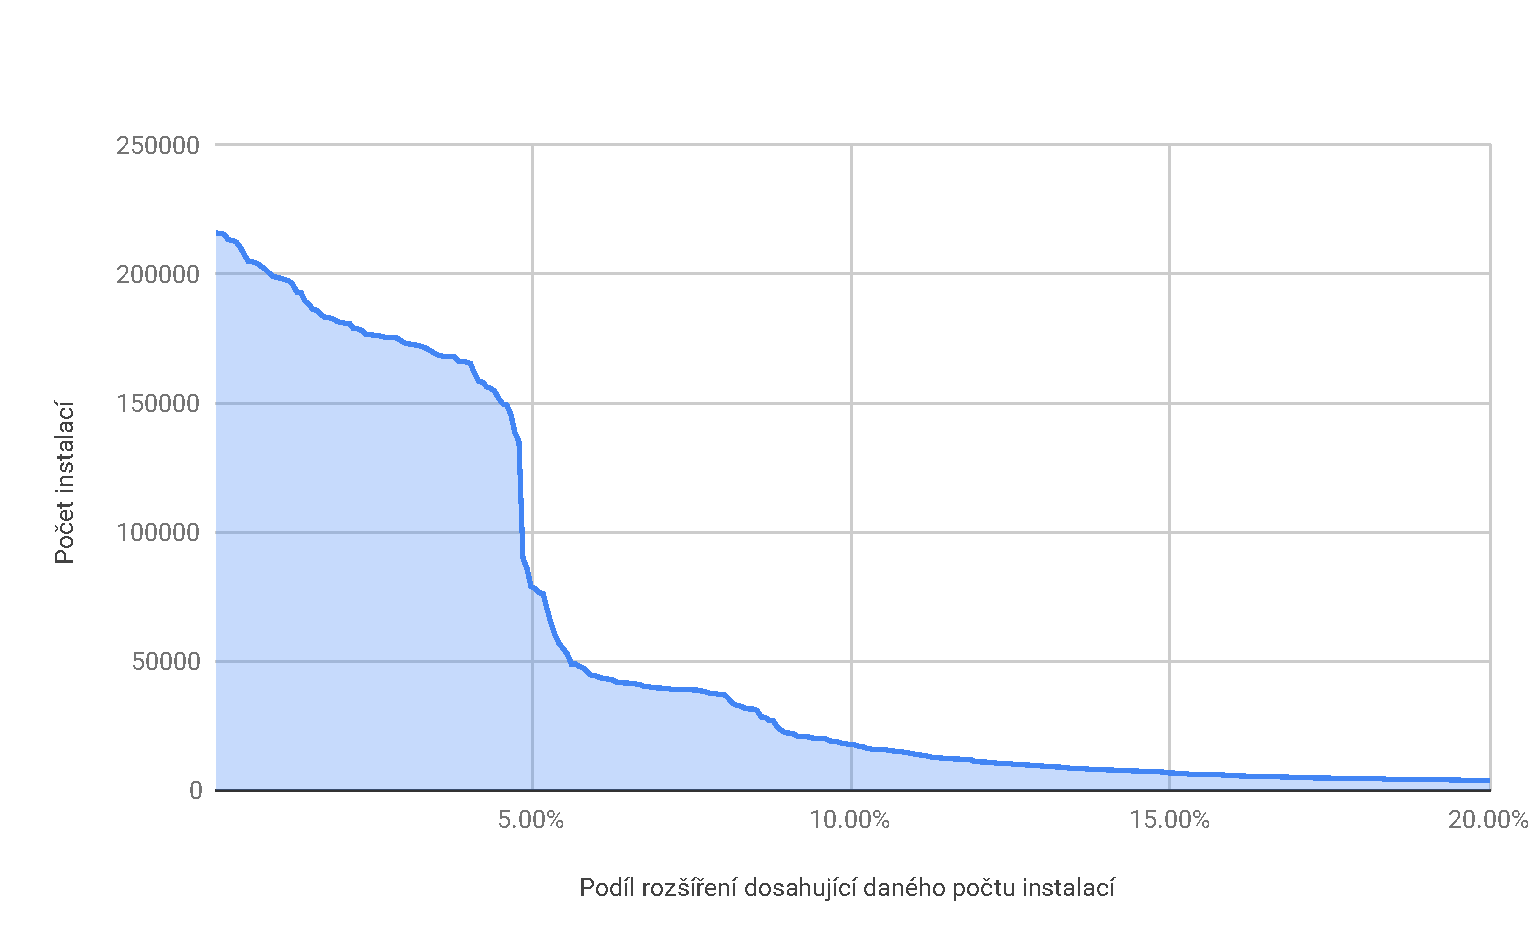
\includegraphics[width=\textwidth,height=9cm,keepaspectratio]{media/jenkins-plugins.pdf}
                    \caption{Rozdělení počtu instalací. Oříznutých 80~\% je klesající dlouhý ocas. Pouze zhruba $80$ rozšíření má víc instalací než $100\,000$. To jsou pluginy, které se nabízí administrátorům při první konfiguraci Jenkins. Necelých $200$ rozšíření má víc než $10\,000$ instalací. Přes 60~\% publikovaných rozšíření má méně než $1\,000$ instalací.}
                    \label{fig:jenkins-plugins}
                \end{subfigure}

                \begin{subfigure}[b]{\textwidth}
                    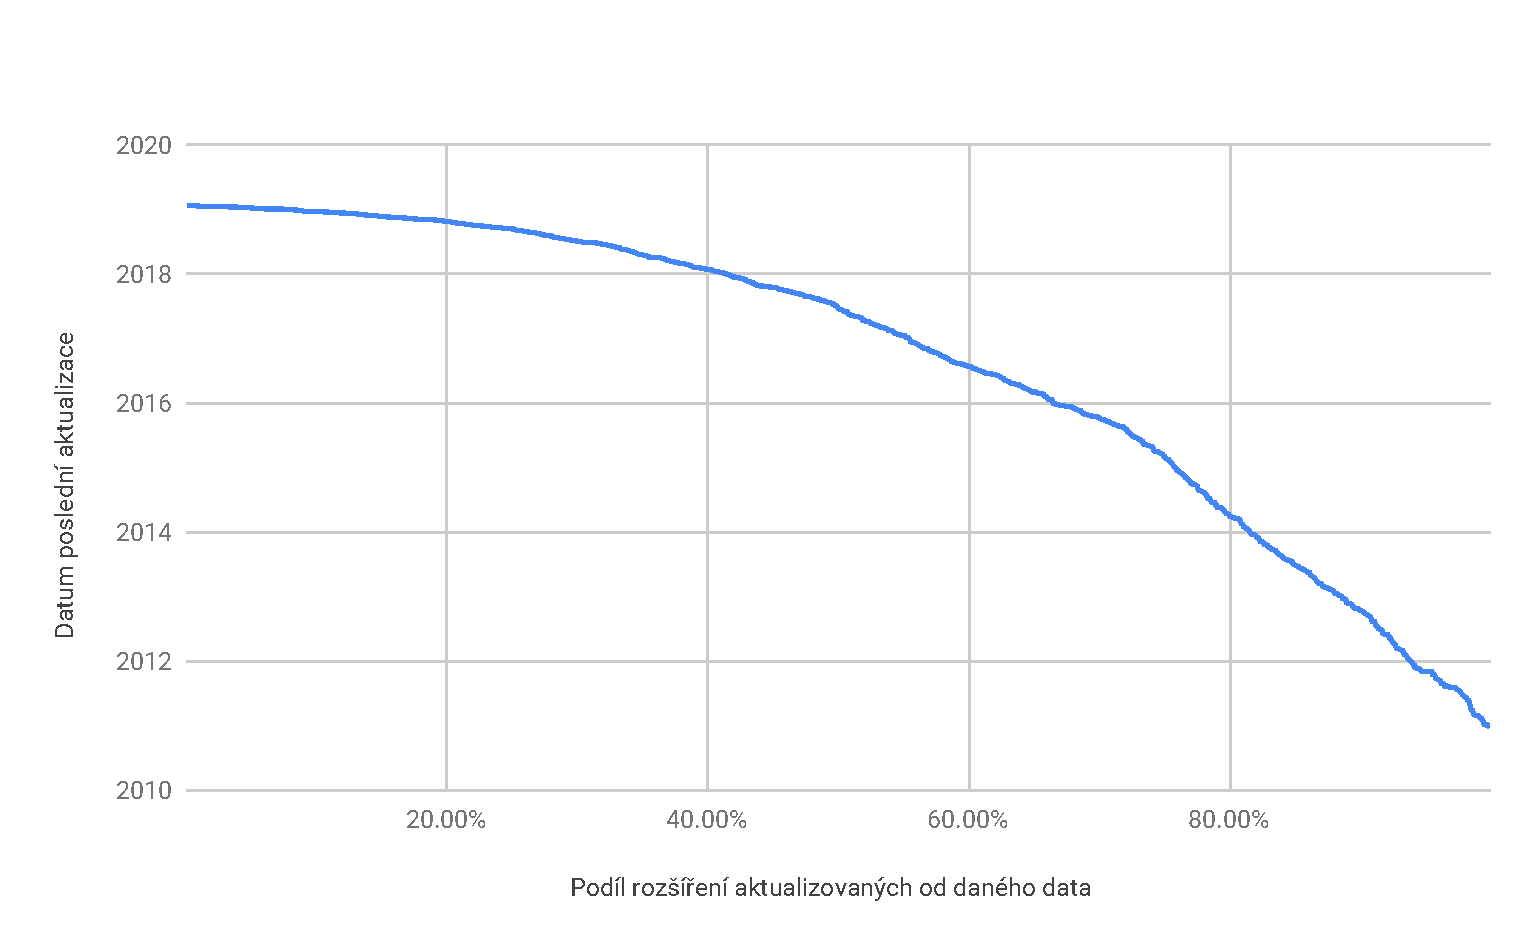
\includegraphics[width=\textwidth,height=9cm,keepaspectratio]{media/jenkins-plugins-update.pdf}
                    \caption{Rozdělení podle poslední aktualizace. Skoro 30~\% byla aktualizována v posledním půl roce. 40~\% rožšíření mělo alespoň jednu aktualizaci za poslední rok.}
                    \label{fig:jenkins-plugins-update}
                \end{subfigure}

                \caption{Zdroj: data vytažena z \url{https://plugins.jenkins.io/}, agregace a vizualizace vlastní. Data jsou dostupná na přiloženém mediu v \code{appendix/jenkins-plugin-*.csv}.}
            \end{iffigure}
            \clearpage
        }

        Celkově působí Jenkins velmi roztříštěně. Některá rozšíření mají dokumentaci na Jenkins Wiki, jiné na portálu Jenkins Plugins a zbytek na vlastních dedikovaných stránkách nebo na GitHubu. Část pluginů má nějaký obsah na všech těchto místech a dohledat konkrétní informace bývá obtížné. Velký problém je poznat, jaká rozšíření nainstalovat. Pipelines jsou pro moderní použití Jenkins nezbytné, ale administrátor to musí sám vyčíst z blogů a odkoukat od ostatních. Je na trhu prostor pro svéhlavou distribuci Jenkins, která by obsahovala \textit{best-practice} rozšíření a konfiguraci.

        Jenkins umožňuje upravit prakticky cokoliv. Na rozdíl od GitLabu, kde vývojář může konfigurovat pipeline a spouštět libovolné procesy, na Jenkins lze upravit samotné rozhraní. Šlo by například rozšířit Jenkins o stránku s přehledem nasazených prostředí, podobně jako má GitLab své Environments. Je pak ale na zvážení, jestli není praktičtější podobně velké úpravy vyčlenit do samostatné webové aplikace. Kromě toho existují rozšíření, které umožňují spouštět skripty v rámci jobů. Například \textit{Pipeline: Groovy} načte zdrojový kód umožňuje ho v jobu spustit. To bývá užitečné pro vyčlenění společné funkcionality napříč několika projekty a pro zpřehlednění pipeline.

    \subsection{Zabezpečení}
        Stejným způsobem kterým Jenkins deleguje funkcionalitu na pluginy, přenáší zodpovědnost i za bezpečnost. Jádro Jenkins mělo za rok 2018 nahlášeno 53 \glstext{CVE}, rozšíření pro Jenkins skoro 100 \cite{cve-jenkins}. Čím víc rozšíření je do Jenkins nainstalováno, tím větší je plocha pro potenciální útočníky.

        Izolace klientů o něco horší než u GitLabu. Přestože oba systémy podporují různé úrovně izolace samotných jobů, nastavení práv pro webovou administraci Jenkins je velmi složité a nepřehledné. Tak jako všechno ostatní deleguje Jenkins i \glstext{ACL} na rozšíření. Základní rozřšíření \textit{Matrix-based security} umožňuje nastavit každému uživateli nebo skupině práva k nějaké akci. Jenom u zdroje \textit{Job} je ale 9 oprávnění a není dobře zdokumentované, co přesně umožňují. Některé integrace, například GitHub, podle dokumentace umožňují dynamicky přiřazovat práva podle uživatelů přiřazených k danému repozitáři. Tuto funkci se mi ale nepodařilo zprovoznit; buď byl projekt úplně veřejný, nebo úplně nedostupný.

        Izolace v rámci samotných agentů/workerů může být perfektní. Je dokonce i možné dynamicky reagovat na využití a zapínat a vypínat agenty v cloudu. Některá rozšíření umožňují využívat i krátkožijící virtuální stroje v cloudu jako je \glstext{AWS} CodeBuild \cite{jenkins-codebuild}.

        \begin{iffigure}
            \centering
            \makebox[\textwidth][c]{
                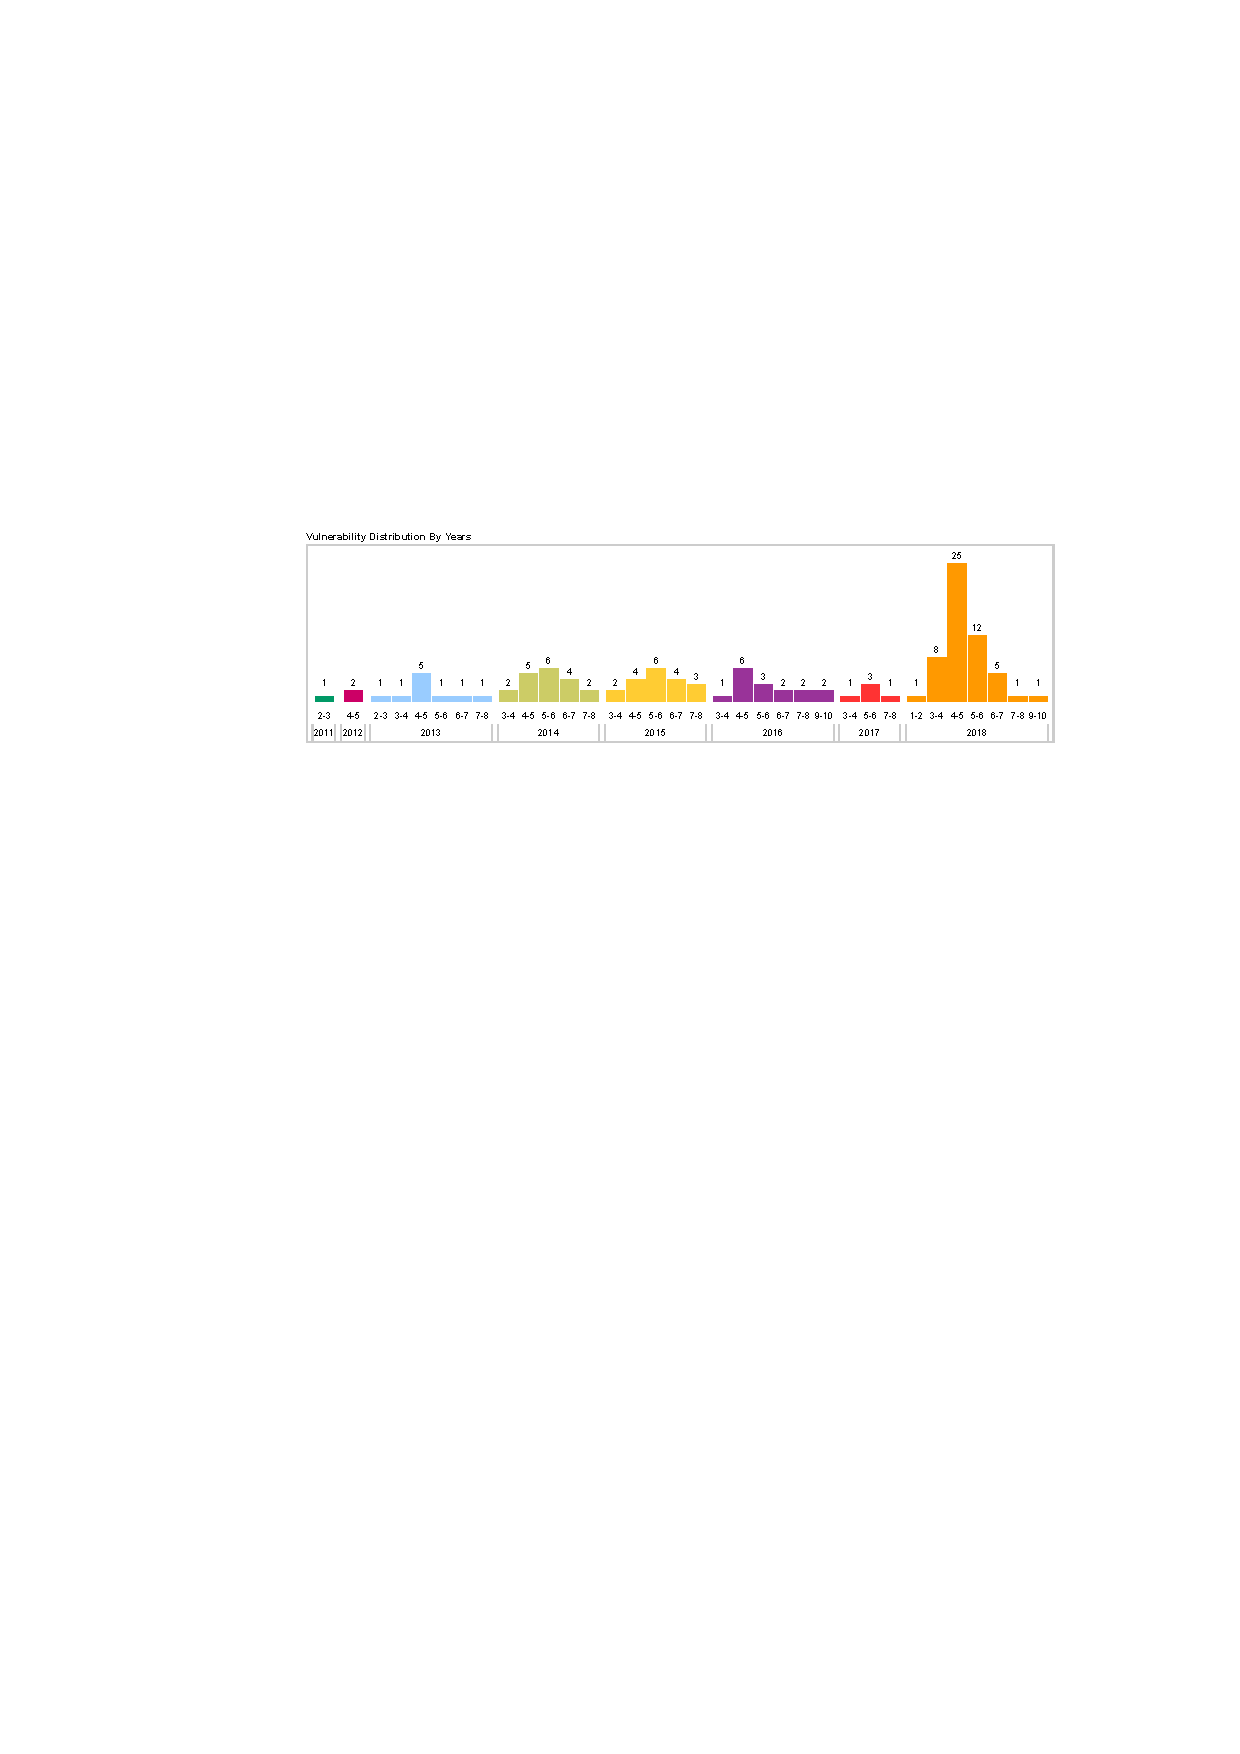
\includegraphics[width=1.2\textwidth]{media/jenkins-cve.pdf}
            }
            \caption{Rozložení Jenkins \glstext{CVE} a přiřazené skóre podle \glstext{CVSS}. Většina nahlášených bezpečnostních chyb bylo \glstext{XSS} a únik informací. Nejvážnější problém v jádru v roce 2018 byla možnost neomezeného spouštění procesů na masteru, které mohl využít každý uživatel s právem přidat nový agent \cite{cve-jenkins}.}
            \label{fig:gitlab-review-cycle}
        \end{iffigure}

    \subsection{Dostupnost}
        Tím že Jenkins je výhradně ke spouštění jobů, dostupnost neřeší. Myšlenka je taková, že Jenkins periodicky skenuje různé repozitáře a při detekci změny začne nový job. V případě výpadku se pouze job zpozdí. Na rozdíl od GitLabu neposkytuje další vývojářům další funkce jako je repozitář verzovacího systému, správa úkolů a podobně. Přesto je výpadek Jenkins problematický i při každodenním užívání: projekty nemůžou využívat spouštění jobů z \glstext{API} a vyvojáři nemůžou zobrazovat logy a využívat artifacts.

        Při instalaci ale i při aktualizaci rozšíření vyžaduje Jenkins restart. Některá rozšíření lze nainstalovat i bez restartu, ale pro upgrade je vyžadován \cite{jenkins-norestart}. Nabízí možnost restartovat po dokončení všech právě běžících jobů, nebo manuální restart. V mém testovacím prostředí trvá restart přes 30 vteřin. Stejně tak je nutný restart při upgrade celého jádra.

        Jenkins je stavová aplikace persistující na disk. Není možné spustit víc replik a sdílet úložiště například přes \glstext{NFS}, protože Jenkins drží část informací jenom v paměti. Nejlepší dostupnosti lze dosáhnout použitím failoveru (\textit{cold standby}). Je nutné zajistit, aby aktivní proces byl nejprve ukončen a persistoval všechny stavy na disk a až poté je možné zapnout standby instanci \cite{jenkins-ha}. Ve výsledku tedy čekáme na vypnutí a zapnutí celé aplikace a doba výpadku je stejně dlouhá jako bez použití failoveru, ale infrastruktura pak není závislá na dostupnosti jednoho datacentra. Stojí za povšimnutí, že tuto formu failoveru získáme bez práce při použití libovolného orchestrátoru kontejnerů (Docker Swarm, Kubernetes, OpenShift, \ldots).

        Pokud se Jenkins restartuje, běžící joby se ztratí. V administraci a v \glstext{API} je možnost \textit{safe restart}, která pozastaví frontu jobů, nechá už běžící joby doběhnout a poté systém restartuje.

        \todo{popsat backup a restore proces}\blind[1]

    \subsection{Integrace}

        \todo{Integrace Jenkins, oznámení na GitHub/GitLab/Bitbucket/\ldots}\blind[2]
        \todo{Možnosti deploy z Jenkins do cílového systému; k8s, sftp, openstack, \ldots}\blind[2]
        \todo{Integrace s Kubernetes, docker v dockeru}\blind[1]

    \subsection{Praktické nasazení projektů}
        \subsubsection{Projekt 1}
            Pro statický projekt jsem připravil pipeline využívající Docker. Kompilace Jekyll zdrojů potřebuje hodně závislostí a je nepraktické je instalovat přímo na hostitelské servery (jak jsem otestoval \pfxref{v sekci o GitLab}{subsec:gitlab-p1}). V Jenkins jsem ručně založil novou Pipeline a v nastavení jsem vybral možnost \textit{Pipeline Script from \glstext{SCM}} -- to umožňuje verzovat Jenkinsfile přímo v projektu. Alternativa je ručně psát pipeline přímo ve webové administraci Jenkins, což odporuje \textit{Infrastructure as a Code}. Dále jsem musel ručně zadat cestu k repozitáři. Narazil jsem na chybu v Jenkins, která znemožňuje v Pipeline klonovat lokální Git repozitáře. Tento problém jsem obešel uvedením vzdáleného repozitáře na GitLabu.

            Samotná deklarativní pipeline není složitá. Uvedl jsem docker obraz, ve kterém se má kompilace provést. Dále jsem rozdělil práci na dvě stages: build a deploy. Stejně jako GitLab umí Jenkins opakovat jednu stage bez nutnosti spouštět znovu celou pipeline, což se hodí pro přechodné chyby, pro deploy, rollback a podobně. V samotných stages se pak spouští předpřipravené scripty, které využívám pro všechna testovaná \CICD prostředí.

        \subsubsection{Projekt 2}
            \todo{[PROGRAMOVANI] Popsat deploy projektu 2 z Jenkins}\blind[2]


        \subsubsection{Projekt 3}
            \todo{[PROGRAMOVANI] Popsat deploy projektu 3 z Jenkins}\blind[2]


    \newpage
    \section{Concourse}
    Concourse je minimalistické \CI. Zjednodušeně řečeno obsahuje pouze tři základní koncepty: pipeline (projekt), job a přihlášení.

    \todo{Concourse záměrně nemá žádné vazby na nic a jediné co podporuje je polling, takže to nefunguje pro spoustu use-cases.}

    \todo{popsat že má skvělou dokumentaci a popisují očekávaný disk, cpu, memory usage i high availability}

    \subsection{Architektura Concourse, možnosti konfigurace}
        Concourse využívá -- podobně jako Jenkins a GitLab -- architekturu kontrolerů (které nazývají \textit{web node}) a pracovních uzlů (\textit{worker node}). Na rozdíl od ostatních systémů ale má všechny části bezstavové. Data se persistují do externí PostgreSQL databáze. Díky tomu lze řídící rovinu libovolně škálovat a při provozu ve víc replikách má výbornou dostupnost.

        \missingfigure[figwidth=\columnwidth,figheight=7cm]{Architektura Concourse \label{pic:concourse-architecture}}
        \todo{\url{https://concourse-ci.org/concepts.html\#component-atc}}

        Nasazení Concourse je skvěle zdokumentované. Podobně jako u dalších distribuovaných systémů je potřeba před spuštěním jednotlivých komponent vygenerovat celou řadu klíčů. Na podepisování uživatelských session a interní komunikaci, identifikátor pro \glstext{SSH} server a pro každý \textit{worker node} jeden klíč k registraci ke kontroleru. Další nastavení je volitelné \code{concourse-cluster}.

        Pro rychlé otestování funkčnosti a drobné projekty nabízí Concourse zjednodušenou variantu spuštění. Jedním příkazem (\code{concourse quickstart}) se spustí kontroler a worker a automaticky se pro ně vygenerují a zaregistrují potřebné klíče.

        Concourse neřeší balancování Web instancí. Je možné -- a dokonce doporučené -- mít víc než jednu repliku kontroleru, ale je na administrátorovi aby příchozí požadavky nějakým způsobem směroval, Concourse pouze na každé Web instanci vystavuje \glstext{HTTP} \code{concourse-cluster}. V Kubernetes, OpenShift nebo podobném orchestrátoru můžeme přímo využít vestavěné služby, pro jiné systémy se ale nasazení Concourse komplikuje přidáním dalšího software pro load balancing.

        Worker instance musí být spuštěné pod root uživatelem. Podle firmy DigitalOcean je to proto, že worker potřebuje spravovat kontejnery \code{concourse-do}. To může v základním nastavení Dockeru ale libovolný linuxový uživatel v \code{docker} skupině. \code{docker-postinstall}. I s přístupem k Dockeru ale Concourse worker odmítal nastartovat a stále vyžadovat root uživatele.

    \subsection{Rozšiřitelnost}
        Oproti Jenkins, kde se instalují pluginy, přistupuje Concourse k rozšiřitelnosti obráceně. Poskytuje několik základních zdrojů (pipeline, job) a \glstext{API}. Uživatelé můžou v rámci spuštěných kontejnerů volat cokoliv potřebují. Alternativní rozhraní a podobně je možné implementovat jako externí aplikaci. Concourse se snaží dělat jednu věc a dělat jí dobře.

        Concourse lze částečně rozšířit přes koncept \textit{resources} (zdroje). Ty se balíčkují jako kontejnery a jediný požadavek na ně je, že musí obsahovat programy \code{check}, \code{in} a \code{out} v cestě \code{/opt/resource} \cite{concourse-resource}. Podle konfigurace konkrétní pipeline se pak periodicky volá \code{check}, který má na za úkol vrátit seznam všech nových verzí. Volání \code{in} a \code{out} má za úkol dostat nějaké informace do Concourse pipeline, resp. je nahrát z pipeline ven. Příklad zdroje může být \glstext{RSS}, kde lze periodicky sledovat feed nějaké závislosti a při vydání nové verze automaticky spustit pipeline. Jiný příklad je zdroj git, který může nejenom reagovat na nové verze, ale i udělat nějaké změny v repozitáři. Resource se může napojit na libovolné \glstext{API} a existují stovky opensource integrací na všechno od monitorovacích nástrojů po \CD systémy jako je Kubernetes/Helm a řada dalších \cite{concourse-resource-list}.

        Protože některé \code{check} operace můžou být drahé a případně pomalé, přišel Concourse s možností definovat pro zdroje také token, kterým lze programově vynutit okamžité spuštění \code{check} z \glstext{API}. To je něco co by používala organizace pracující aktivně na několika málo z hodně repozitářů, kde je žádoucí spustit pipeline do pár vteřin od změny, ale není praktické s takovou periodou kontrolovat desítky repozitářů.

    \subsection{Zabezpečení}
        \label{subsec:concourse-security}
        \todo{Každý v týmu může dělat cokoliv? Ověřit}\blind[1]
        \todo{Jaké jsou historická CVE? Jaká je izolace klientů? Co aplikace potřebuje za přístupy?}\blind[2]

    \subsection{Dostupnost}
        \todo{Může Concourse běžet ve víc replikách? Jak se dělá upgrade? Jak stabilní to je?}\blind[3]

    \subsection{Integrace}
        \todo{má to integrace na spoustu oauth (a obecně auth) viz concourse quickstart --help}\blind[1]
        \todo{\url{https://medium.com/concourse-ci/designing-a-dashboard-for-concourse-fe2e03248751}}
        \todo{Integrace Concourse, oznámení na GitHub/GitLab/Bitbucket/\ldots}\blind[1]
        \todo{Možnosti deploy z Concourse do cílového systému; k8s, sftp, openstack, \ldots}\blind[1]

    \subsection{Praktické nasazení projektů}
        Navzdory skvělé dokumentaci pro nasazení Concourse clusteru bylo pro mě vytváření pipeline a jejich správa utrpení. Na rozdíl od ostatních \CI není kanonická verze pipeline v repozitáři, ale v Concourse. To souvisí s tím, že concourse je hodně abstraktní a nesoustředí se jenom na stavbu aplikací. Existují zdroje \cite{concourse-pipeline-res} které umožňují pipeline editovat, ale použití by reálně znamenalo vytvořit jednu pipeline která by byla „napevno“ nastavená v concourse a stahovala aktuální stav repozitáře, upravila by jinou pipeline podle specifikace a následně danou pipeline spustila. Výsledek je zbytečně komplikovaný a pomalý.

        Pipeline se tak zakládají a upravují z konzole, ne úpravou konfigurace v repozitáři a pushnutí, takže systém nenutí vývojáře specifikaci pipeline verzovat.

        Pro mě nejvíc zmatená část Concourse je koncept \textit{task}. Tasky umožňují spustit část pipeline ze staženého resource (což může být repozitář, ale i cokoliv jiného). Lze tak drobnou část pipeline editovat jenom s přístupem k repozitáři, ale v tasku nelze nastavit definici resources, jejich stažení ani jejich nahrání. Tasky mají vstup a výstup, ale jejich integrace do pipeline se řeší mimo. Po praktické zkušenosti s nasazením všech tří projektů mi toto řešení přijde míň vhodné, než mít kompletní definici pipeline v jednom souboru spravovaném přes konzoli.

        %\todo{že při vytvoření pipeline to bylo pauznuté a nešlo to z UI vyřešit a musel jsem hledat command}

        \subsubsection{Projekt 1}
            Při nasazení projektu jsem se potýkal s náhodnýmy problémy, které ostatní \CI systémy neměly. Jedna z chyb byla například kryptická zpráva \textit{volume graph is disabled}. To je známá chyba už z roku 2016 a je o tom, že v dokumentaci je uveden klíč \code{image} ale Concourse očekává \code{image_resource} \cite{concourse-issue-402}. Banalita, ale při kombinaci se špatnou zastaralou dokumentací a malou komunitou je to zdlouhavý problém k řešení. Další problém který jsme při implementaci měl bylo stahování Docker kontejnerů z veřejného repozitáře. Přestože jsem nejnovější Concourse spustil na čisté \glstext{VM} přesně podle dokumentace, bylo pravděpodobně nastaveno špatně \glstext{DNS}. Po ruční editaci nameserverů jsem skončil na další kryptické chybě \code{unknown handle: \textit{uuid}}. Na to nepomohlo ani smazat celou pipeline a vytvořit ji znovu. Rozhodl jsem se smazat celou databázi a začít znovu. Pro testování je to bezproblémové řešení, ale Concourse mě tímto hodně odlákal a v produkčním prostředí mu nedůvěřuji. Ještě na další problém jsem narazil po restartu, kde se nějakým záhadným způsobem poškodil stažený Docker obraz a Concourse končil chybou, ale nestáhnul obraz znovu.

            Pro kompilaci projektu a nahrání výsledků na web server jsem využil dva zdroje. Prvního zabudovaný zdroj \code{git} sleduje repozitář projekty a při detekci změny spustí zbytek pipeline. Následně se v jobu repozitář naklonuje a v rámci tasku se spustí kompilace. Výsledné vystavěné soubory se pak posílají do zdroje \code{rsync-resource}, který je definovaný externím Docker obrazem. Přijatá data nahraje přes rsync na server.

            V ukázkových definicích jsem vědomě zapsal soukromé klíče přímo v plaintextu. Concourse podporuje různé systémy pro předávání tajemství a popisuji je \pfxref{v sekci}{subsec:concourse-security}. Nasazení těchto produktů a jejich použití bylo ale mimo rozsah této práce.

        \subsubsection{Projekt 2}
            \todo{Popsat deploy projektu 2 z Concourse}\blind[2]

        \subsubsection{Projekt 3}
            \todo{Popsat deploy projektu 3 z Concourse}\blind[2]


    \newpage
    \section{Drone}
    Drone je minimalistické \CI postavené na kontejnerech. Je to svým způsobem jenom Docker orchestrátor, který má navíc drobné webové rozhraní. V \glstext{UI} lze dělat pouze dva úkony: číst výstup jobů a zapínat/vypínat sledování repozitářů. Kromě toho je celý web implementovaný jako \glstext{SPA}. To má sice pozitivní vliv na rychlost přepínání stránek, ale při testování občas aplikace nereagovala a několikrát se zasekla úplně. Dokonce ve webové administraci není ani seznam agentů, joby čekající na zpracování a podobně.

    Některé důležité funkce skrývá Drone za placenou licenci. Nejde ani o korporátní podporu, ale o nezbytné vlastnosti bez který lze \CI těžko provozovat. Mezi ně patří: dynamický runner, který by umožňoval využívat cluster nebo externí služby (například \glstext{AWS} CodeBuild) podle vytížení; sdílení tajemství napříč organizací a obecně podpora pro externí správce tajemství; šablony pro pipeline.

    \subsection{Architektura Drone, možnosti konfigurace}
        Dokumentace Drone je dostatečně obsáhlá, ale není vyčerpávající a odkazy jsou navíc netypicky pojmenované. Instalace je rozdělena podle externího správce úložišť, tradičně bývá odlišná dokumentace pro způsoby instalace (bare metal, kontejnery, \ldots). Není možné v jedné Drone instanci využívat zároveň například GitLab a Bitbucket, podporováno je pouze jedno úložiště. Dokumentační stránka o instalaci na Kubernetes je dokonce úplně špatně. Doporučuje spouštět Drone server jako \code{Pod} (mělo by jít o \code{Deployment}, nebo Helm chart) a agenti dokonce naprosto chybí. Další problém dokumentace je, že používá ve všech ukázkách Docker obrazy bez tagu. To je špatně, protože výchozí tag \code{latest} se může kdykoliv změnit na nekompatibilní verzi. Vždy je lepší explicitně uvést tag.

        Stejně jako ostatní \CI se Drone skládá z jednoho masteru a agentů. Master persistuje data do sqlite databáze, ale některá data o frontě požadavků udržuje pouze v paměti \cite{drone-ha}. Nemá žádné externí závilosti.

    \subsection{Rozšiřitelnost}
        Drone rozlišuje dva koncepty. První jsou \textit{pipeline plugins}, což jsou obyčejné kontejnery spuštěné v pipeline. Jediný rozdíl je drobné syntaktické zjednodušení, které umožňuje v konfiguraci pipeline psát místo \code{environment[PLUGIN\_KEY]=x} jenom \code{settings.key=x}. Kdyby Drone tuto funkci neměl, byla by tvorba pluginů transparentnější a přístupnější i těm nejméně zkušeným uživatelům.

        Druhý koncept rozšíření -- dostupný pouze v placené Enterprise verzi -- upravuje nějakým způsobem definici pipeline. Jediné zdokumentované rozšíření je zatím Jsonnet, které umožňuje používat stejnojmenný šablonovací jazyk místo \glstext{YAML} \cite{drone-jsonnet}.

    \subsection{Zabezpečení}
        Díky kontejnerové architektuře má Drone základní izolaci i v rámci jednoho agenta. Lepší izolace lze dosáhnout v placené verzi, která nabízí dynamické agenty, které můžou spouštět \glstext{VM} nebo nějakým způsobem využívat cloud.

        Vynikající vlastnost kterou ostatní v základu \CI nenabízejí je možnost zašifrovat tajemství a umístit ho do veřejně čitelné pipeline. Využívá se k tomu asymetrické šifrování, při kterém \CI nikdy nezveřejňuje svůj privátní klíč. Dál je podporován mj.~HashiCorp Vault a \glstext{AWS} Secrets Manager.

        Při napojení na GitHub je vyžadováno moc práv, včetně čtení a zápisu do všech soukromých repozitářů. Je na to otevřené issue od začátku roku 2018, ale Drone je zatím bez opravy \cite{drone-github-acl}.

        Nenašel jsem žádná Drone \glstext{CVE}, ani jsem nenašel žádné zdokumentované bezpečnostní problémy ve veřejném seznamu chyb a úkolů celé Drone organizace (ať otevřené, nebo vyřešené).

    \subsection{Dostupnost}
        Podobně jako ostatní \CI má Drone jeden stavový master, který není možné load balancovat. Jeden z autorů prohlásil, že na stabilním cloudu má Drone uptime $99,999$~\%~\cite{drone-ha}. Není ale možné, aby zahrnoval i aktualizace. Kromě toho s nástupem smýšlení \textit{Infrastructure as Code} není běžné udržovat dlouhožijící \textit{pet} servery.

        \todo{[PROGRAMOVANI] Jak se dělá upgrade? Jak stabilní to je?}\blind[1]
        \todo{[PROGRAMOVANI] Jak se dělá backup/restore}\blind[1]

    \subsection{Integrace}
        Drone podporuje jenom vybrané správce repozitářů: GitHub, Gitlab, Bitbucket, Gitea a Gogs. Důležité je, že neexistuje podpora pro obecný git remote.

        Ani přes úzkou integraci na repozitáře není ale výsledná integrace bezchybná. Například oznámení výsledku pipeline na GitHub (tzv. \textit{Commit Status} nebo novější \textit{Checks}) nejsou zabudované a je nutné použít plugin, což dále komplikuje pipeline kterou uživatel musí napsat a udržovat.

        \todo{Možnosti deploy z Drone do cílového systému; k8s, sftp, openstack, \ldots}\blind[1]

    \subsection{Praktické nasazení projektů}
        \subsubsection{Projekt 1}
            Pro statický projekt jsem jako u ostatních \CI vytvořil dvoukrokovou pipeline, kde první část kompiluje zdrojové soubory nástrojem Jekyll a druhá část nahrává výsledný web na webový server pomocí \code{rsync}. Protože všechny kroky běží v kontejneru a nelze použít zdroje na hostitelském stroji, místo přednahrání \glstext{RSA} klíče je nutné ho umístit do pipeline. Aby byl dostupný pouze pro \CI a nemohl ho nikdo jiný zneužít, je zašifrovaný \glstext{CLI} nástrojem \code{drone encrypt}. Tato utilita nepodporuje načítání z \code{stdin}, takže binární, víceřádkové nebo obecně složitější data je nutné nějakým způsobem překódovat. V tomto případě jsem klíč nejprve překódoval s \code{base64}. Toto řešení není ideální, protože vyžaduje práci v kontejneru, kde dekódovací nástroj nemusí být nainstalovaný.

            Další problém na který jsem při tvorbě pipeline narazil byla chybějící indikace stavu pipeline ve webovém rozhraní. Při prvním dlouhém stahování docker obrazu pro danou pipeline vypadá Drone rozbitě/zaseknutě. Chybí jakákoliv indikace postupu nebo dokonce času k dokončení.

            Přes všechny počáteční nesnáze je konfigurace Drone pipeline relativně snadná a přímočará. Především tomu pomáhá koncept \textit{Volumes}, což definuje složku souborů sdílející se mezi všemi joby. Ostatní \CI toto řeší mnohem složitěji, například přes read-only \textit{artifacts}.

        \subsubsection{Projekt 2}
            \todo{[PROGRAMOVANI] Popsat deploy projektu 2 z Drone}\blind[2]

        \subsubsection{Projekt 3}
            \todo{[PROGRAMOVANI] Popsat deploy projektu 3 z Drone}\blind[2]


    \newpage
    \section{GoCD}
    Systém GoCD vychází z~projektu Cruise~\cite{thoughtworks-gocd}. Oba projekty vznikly ve firmě ThoughtWorks, kde pracoval průkopník a zastánce praktik \textit{extrémního programování} M. Fowler~\cite{fowler-go}. Fowler systém Cruise doporučoval ve známém článku o~\CI~\cite{fowler-ci}.

    \subsection{Architektura GoCD, možnosti konfigurace}
        GoCD stejně jako většina ostatních \CI staví na architektuře jednoho kontrolního serveru a řadě interních nebo externích agentů, které se starají o~spuštění jednotlivých jobů. Ve výchozím nastavení jsou data persistována v~embedované H2 databázi na server procesu. Instalace GoCD je díky tomu jednoduchá, protože stačí zaregistrovat externí repozitář a nainstalovat balíček pro server a pro agenty.

        Po prvním zobrazení webového rozhraní serveru se zobrazuje quick-start, který provádí vytvořením nové pipeline. Přestože GoCD podporuje \textit{Pipelines as code}, očekávaný primární vstup je klikání v~administraci~\cite{gocd-pas}. Načítání externích souborů je vyřešeno rozšířením, jehož použití se definuje v~hlavní \glstext{XML} konfiguraci na webu. Separovaná konfigurace tak není kompletní a závisí na další ruční konfiguraci.

    \subsection{Rozšiřitelnost}
        GoCD nabízí několik možností, jak rozšiřovat výchozí funkcionalitu pomocí pluginů~\cite{gocd-extensions}. Na rozdíl od Jenkins, kde lze upravit prakticky cokoliv, vystavuje pro pluginy GoCD jenom některá \glstext{API}. Nelze tak například ovlivňovat uživatelské rozhraní.

        Zhruba 80 pluginů je na oficiálním registru~\cite{gocd-plugins}. ThoughtWorks~Inc.~zaštiťují 8 pluginů a a z~toho je 6 placených.

        Z~veřejně dostupných rozšíření jsou všechna kromě jednoho hostována na GitHub. Jak jsem ale vizualizoval \pfxref{v~grafu}{fig:jenkins-plugins}, GoCD rozšíření jsou ještě hůř udržovaná než ta pro Jenkins. A~to je jich méně než dvacetina.

        \begin{iffigure}
            \centering
            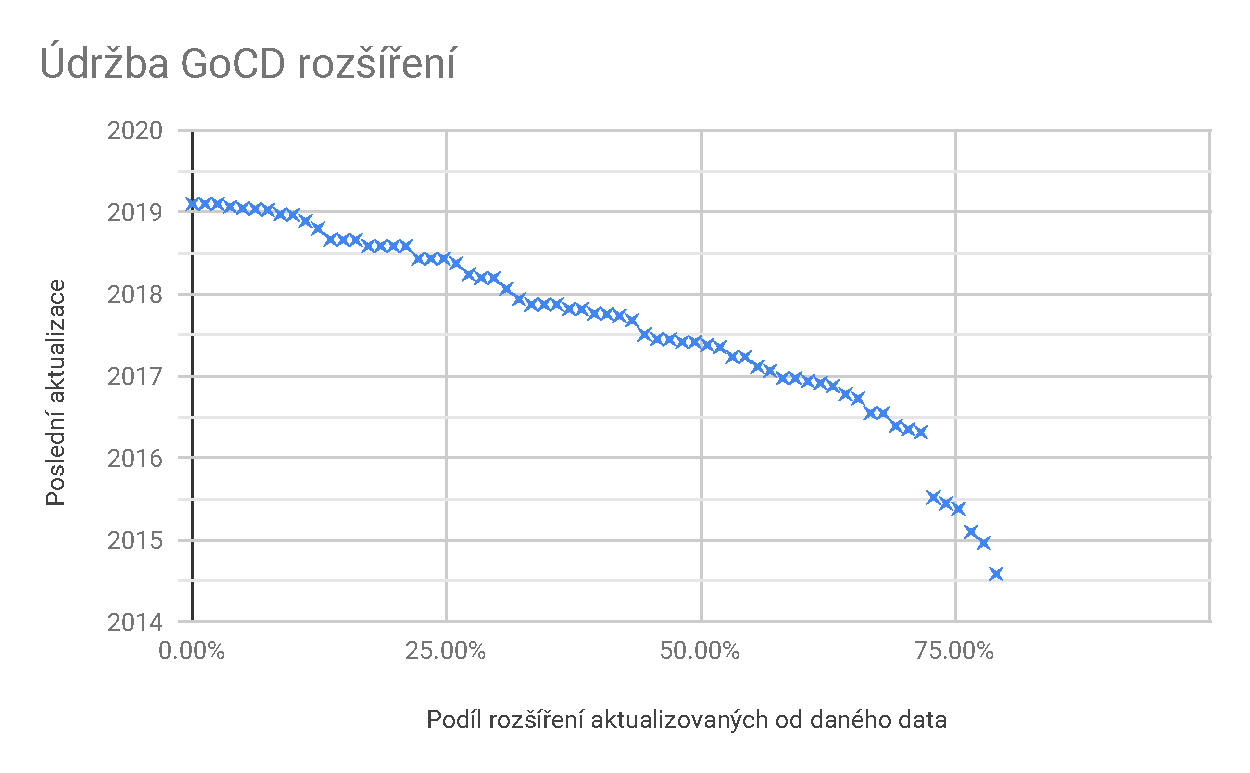
\includegraphics[width=\textwidth,height=9cm,keepaspectratio]{media/go-plugins-update.pdf}
            \caption{Rozdělení podle poslední aktualizace. Pouze 17 rozšíření (20 \%) bylo aktualizováno v~posledním půl roce. Pouhých 30~\% rozšíření mělo alespoň jednu aktualizaci za poslední rok. Přibližně 20 \% rozšíření nemá žádné stabilní vydání. Zdroj: data vytěžena z~GitHub repozitářů, dostupná na přiloženém mediu v~\code{appendix/gocd-plugins.csv}.}
            \label{fig:jenkins-plugins}
        \end{iffigure}

    \newpage
    \subsection{Zabezpečení}
        Po instalaci serveru je v~základu celá administrace dostupná pro všechny, bez autorizace. Lze zapnout zabudovaná rozšíření, která zprovozní přihlášení heslem a nebo přes \glstext{LDAP}. Nic v~\glstext{UI} k~tomu ale správce nenabádá. Velmi překvapivě ale není v~Shodan databázi žádná nezabezpečená instance GoCD na výchozím portu~\cite{shodan-gocd}.

        Izolace klientů závisí na použitých agentech. Klasický agent používá sdílené prostředí a zdroje, ale GoCD podporuje tzv.~\textit{Elastic Agent}, které se zapínají a vypínají dynamicky podle poptávky. Lze je využít pro zapnutí nového prostředí v~Dockeru, Kubernetes, OpenStacku a několika dalších. Tato jednorázová prostředí nabízí lepší izolaci. Nenašel jsem rozšíření, které by dokázalo spravovat Elastic Agents pro VMware nebo jiný virtualizační nástroj, který by měl ještě lepší izolaci klientů.

        Na webu \glstext{CVE} Details jsem pro GoCD nenašel žádná historická \glstext{CVE}. Projekt ale využívá platformu HackerOne, kde za poslední tři roky zpracovali 39 nahlášených chyb~\cite{gocd-hackerone}. Ze zveřejněných reportů je vidět, že správci reagují rychle a bezpečnostní chyby opravují v~co nejkratším možném termínu.

    \subsection{Dostupnost}
        GoCD agenti jsou z~principu stavové aplikace a stejně jako u~všech ostatních \CI jejich výpadek způsobí, že přijdeme o~spuštěné joby. Může jich ale běžet mnoho a pomocí rolling update je lze aktualizovat bez výpadku.

        Server je bohužel také stavový a může běžet pouze v~jedné replice. GoCD prodává velmi drahý \textit{Business Continuity Addon}, který dokáže udržovat standby repliku~\cite{gocd-ha}. Failover proces ale není nijak automatizovaný a povýšení na primární repliku vyžaduje restart GoCD serveru. U~GoCD nelze udělat perfektní HA bez ztráty žádného požadavku když vypadne primární replika.

        Upgrade serveru na novější verzi vyžaduje restart a tím pádem nedostupnost celého prostředí. Navíc se při startu nové verze aplikace automaticky spustí databázové migrace, které na větších instancích podle dokumentace mohou trvat přes 10 minut~\cite{gocd-upgrading}. Celkově je tak při rutinní aktualizaci potřeba počítat s~výpadkem minimálně 15 minut.

        GoCD má jednoduchý proces pro vytvoření zálohy, který lze spustit buď z~\glstext{UI} nebo z~\glstext{API}~\cite{gocd-backup}. Záloha obsahuje dump databáze, vyklikané \glstext{XML} konfigurace aplikace a konfigurace repozitářů, nastavení webového serveru a klíče. Nejsou zálohovány historie a výstupy spuštěných úloh, ani nainstalovaná rozšíření! Proces vytváří archiv na disku aktuálního serveru, který je poté dobré zmigrovat na nějaké externí úložiště.

    \subsection{Integrace}
        Lze propojit GoCD s~dalšími nástroji; některé funkce -- především ty co mají vliv na \glstext{UI} -- jsou vestavěné. To je například odkazování na externí správu úkolů podle regulárního výrazu. Ostatní integrace jsou dostupná jako rozšíření, která je nutné doinstalovat: mezi ně patří například oznámení stavu na GitHub/Stash/Gerrit a podobně. Pro Bitbucket ani Gitlab podpora neexistuje. Lze ji ale doprogramovat jako nové rozšíření.

    \begin{figure}[H]
        \centering
        \begin{minted}[frame=lines,framesep=2mm,linenos]{xml}
<?xml version="1.0" encoding="utf-8"?>
<pipeline name="p2">
  <materials>
    <git url="file:///src/p2-dynamic/" shallowClone="true" />
  </materials>
  <stage name="BuildStage">
    <jobs>
      <job name="BuildJob">
        <tasks>
          <exec command="make">
            <arg>build</arg>
            <runif status="passed" />
          </exec>
          <exec command="make">
            <arg>deploy</arg>
            <runif status="passed" />
          </exec>
        </tasks>
      </job>
    </jobs>
  </stage>
</pipeline>
        \end{minted}
        \caption{Přestože GoCD je primárně určeno ke konfiguraci z \glstext{GUI}, lze editovat přímo konfigurační \glstext{XML} soubory. Vzhledem k chybějící izolaci úkonů v tomto \CI byla tato pipeline navržena jako prosté spuštění dvou příkazů.}
    \end{figure}


        Navzdory svému jménu nenabízí GoCD žádnou podporu pro continuous deployment. Ve webovém rozhraní (ani jinde) není možnost spravovat nasazená prostředí a verze aplikací, podpora pro ručně potvrzené kroky je velmi limitovaná, a integrace s~Kubernetes/OpenShift nebo jiným  nebo neexistuje.

    \subsection{Praktické nasazení projektů}
        \subsubsection{Projekt 1}
            Nasazení GoCD pro statický projekt bylo vesměs stejné, jako u~GitLab shell executoru: na server jsem předinstalovat Ruby a v~rámci pipeline se pak pouze volá instalace Ruby gems a samotná kompilace. Narazil jsem na drobný problém při použití \glstext{RVM} (správce Ruby verzí), který dynamicky upravuje \code{\$PATH}, ale GoCD tato nastavení nerespektoval. Musel jsem tak ručně cestu k~Ruby upravit v~souboru \code{.profile} a restartovat GoCD agent aby se změny projevily.

        \subsubsection{Projekt 2}
            Pro druhý ukázkový projekt byla implementace v~GoCD velmi jednoduchá, protože jsem závislosti předinstaloval při tvorbě prostředí. Pro víc projektů je to nepraktické řešení, ale pokud bude v~systému vždy pouze jeden projekt využívající dané knihovny a podpůrný software, nenarazíme na skoro žádné problémy. Obtížnější az neřešitelné může být testování zároveň několika verzí závislostí (například současná stabilní verze a nejnovější nestabilní verze).

        \subsubsection{Projekt 3}
            Při implementaci \CI pro kontejnerizovaný projekt jsem narazil na to, že GoCD neinterpoluje proměnné prostředí. Je tak nutné explicitně volat \code{sh -c "\$CMD"}, což je zbytečná komplikace bez jasných výhod. Dále jsem se potýkal s~tím, že GoCD nedefinuje běžné proměnné prostředí. Konkrétně \code{CI\_COMMIT\_SHA} je dostupné jen pod názvem \code{GO\_REVISION}. Přes tyto nedostatky poskytuje GoCD možnosti pro kompilaci a nasazení kontejnerizované aplikace.


    \newpage
    \newcommand{\circleci}{\xspace{}CircleCI\xspace}
\newcommand{\travis}{\xspace{}Travis~\glstext{CI}\xspace}
\newcommand{\semaphore}{\xspace{}Semaphore~\glstext{CI}\xspace}

\section{\glstext{SaaS}: \circleci, \semaphore, \travis}
    V této sekci shrnu výhody a nevýhody moderních \glstext{SaaS} \CI. Vyzdvihnu významné rozdíly, pokud na nějaké narazím, ale primárně budu popisovat \circleci, \semaphore a \travis dohromady.

    \subsection{Architektura SaaS CI a možnosti konfigurace}
        \travis a \semaphore mají prakticky z pohledu uživatele prakticky stejnou architekturu. Pro každý job zapnou samostatný virtuální stroj. \travis poměrně překvapivě přešel v roce 2019 kompletně na virtuální stroje; dříve umožňoval spouštět i Docker kontejnery, což využívalo 45 \% všech jobů \cite{travis-arch}. \travis jako důvod uvádí složitější kompilace Docker obrazů pomocí \glstext{DinD}. To ale může znamenat, že pro firmu je to dražší řešení na podporu, ne nutně že jde o lepší řešení pro uživatele. V rámci virtuálního stroje má uživatel veškerou volnost a může instalovat a spouštět vesměs cokoliv. V základním obrazu je předinstalovaná celá řada často používaných nástrojů a runtime ve spoustě verzí. Velmi praktická funkce \travis, kterou ostatní \CI nástroje v základu nemají, je \textit{Build Matrix}: uživatel specifikuje různé verze různých závislostí a \CI pak spustí job pro \textit{všechny} kombinace \cite{travis-build-matrix}. Některé kombinace lze navíc označit jako volitelné a jejich selhání je jenom informační. To se hodí pro předběžné testování nestabilních \glstext{RC} verzí závislostí a podobně.

        \circleci naopak v roce 2018 zmigroval všechny uživatele z virtuální strojů (\circleci 1.0) na čistě kontejnerové prostředí (\circleci 2.0) \cite{circle-migration}. V specifikaci pipeline uživatel uvádí všechny kontejnery které chce spustit a jejich prolinkování/pořadí. Umí také spustit některé služby paralelně a na pozadí, což se používá například pro databáze a podobné závislosti.

         \begin{iffigure}
            \centering
            \makebox[\textwidth][c]{
                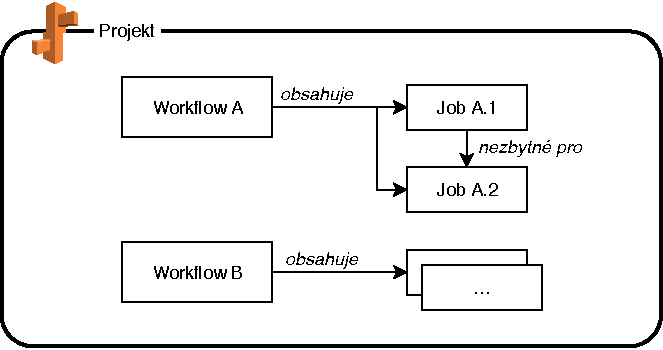
\includegraphics[width=1.0\textwidth]{media/circleci-arch.pdf}
            }
            \caption{Architektura \circleci. Každý projekt může mít několik \textit{workflows}, uvnitř které je libovolný souvislý acyklický graf \textit{jobs}.}
            \label{pic:circle-architecture}
        \end{iffigure}

        \semaphore kombinuje architekturu dvou předchozích řešení: jednotlivé joby běží ve virtuálních strojích, ale jsou provázané přes koncept bloků a data si předávají přes cache. Oproti \circleci chybí možnost zrychlit přípravu prostředí a předinstalaci závislostí Docker obrazem a přitom je na \semaphore definice pipeline výrazně složitější, než na \travis.

    \subsection{Zabezpečení}
        Ani jeden z těchto \glstext{SaaS} \CI systémů nenabízí bug bounty. Pro \travis jsem našel jednu zprávu o bezpečnostní chybě z roku 2018 \cite{travis-db-drop}. Pro \circleci ani \semaphore jsem žádné zveřejněné incidenty nenašel.

    \subsection{Dostupnost}
        \circleci, \travis ani \semaphore nedefinují žádné \glstext{SLA}. Za posledních 12 měsíců měl \circleci uptime $99.90$~\%~\cite{circle-uptime}, \travis $99.93$~\%~\cite{travis-uptime}. \semaphore reportuje za poslední rok podezřele vysoký uptime $100$~\%~\cite{semaphore-uptime}.

        Kromě samotných \CI služeb jsou ale tyto služby závislé na dostupnosti úložišť kódu (GitHub, GitLab, Bitbucket, …).

    \subsection{Rozšiřitelnost}
        Pro \glstext{SaaS} řešení nelze uvažovat systémy pluginů a rozšíření. Veškerá funkcionalita služby musí být přímo integrovaná v systému. Tyto možnosti popisuji v následující podsekci.

    \subsection{Integrace}
        \travis lze používat pouze s repozitáři na GitHub, \circleci a \semaphore podporují kromě toho také Bitbucket. Nelze používat vlastní repozitáře a jiné systémy. Teoreticky lze vytvořit vlastní obálku nad cizím \glstext{API} a posílat webhooky ve formátu jako GitHub, ale nejde o oficiálně podporovanou variantu.

        \semaphore má složité zakládání nového repozitáře. Na rozdíl od ostatních dvou \CI je nutné nainstalovat na klientu spustitelný program, který podporuje pouze Linux a macOS a instaluje se přes \code{curl|bash}. Poté se v repozitáři musí zavolat \code{sem init}, který ale funguje pouze pokud má projekt nastavený \code{origin remote} na GitHub. Běžně stačí projekt přidat v administraci \CI: díky propojení na GitHub \CI ví, jaké projekty existují.

        Všechny tři \CI podporují GitHub perfektně a i nově zveřejněné funkce implementují rychle.

    \subsection{Praktické nasazení projektů}
        \subsubsection{Projekt 1}
            Ze všech \CI vyzkoušených v této práci bylo nasazení na \travis suverénně nejjednodušší. Na deseti řádcích se přehledně definují všechny závislosti a volá se build. I nezaškolený uživatel by dokázal vytvořit novou pipeline podle minimální ukázky.

            Na \circleci je konfigurace pipeline znatelně složitější. Rozdělením na kontejnery se ale separují jednotlivé závislosti a správa komplexních projektů by byla jednodušší. Další výhoda \circleci pro tento projekt je možnost opakovat pouze jenom dílčí kroky a ukládat mezivýsledky do cache, která se může použít při každém spuštění. Toho jsem využil pro instalaci závislostí z Gemfile. Alternativou bylo vytvořit nový Docker obraz a Ruby gemy tam předinstalovat. To má ale řadu nevýhod, předně to zvyšuje komplexitu a bylo by složitější použít jiné gemy (jiná rozšíření pro Jekyll).

            Pro \semaphore jsem de facto musel zkombinovat obě předchozí řešení: v \glstext{VM} jsem nechal nainstalovat Ruby gemy a uložil je do cache. V druhém jobu se cache stáhne a spustí se kompilace samotného statického webu.

            Na rozdíl od ostatních nasazení jsem při testování \glstext{SaaS} neimplementovat celou \CI pipeline včetně nahrání na cílový server. Všechny systémy jsem zprovoznil v lokálním virtuálním prostředí na které není vhodné dělat vzdálený přístup. Místo \code{make deploy} je tak v definicích pouze job s hláškou, kde by se deploy spouštěl.

        \subsubsection{Projekt 2}
            Pro druhý ukázkový projekt jsem upravil konfigurace vytvořené pro statickou aplikaci. Pro \circleci a \travis jsem finální funkční pipeline vytvořil na první pokus. Pro \semaphore bylo z dokumentace nutné nastudovat, jaké obrazy pro \glstext{VM} jsou dostupné a případně jaké jsou poskytované nástroje jsou instalaci a konfiguraci závislostí. Konkrétně pro \glstext{PHP} je předinstalován nástroj phpbrew. Dále jsem musel ladit nastavení cache složky \code{vendor} ve které jsou závislosti nainstalované nástrojem \code{composer}, především aby fungovalo sdílení dat mezi krokem pro kompilaci a pro nasazení.

        \subsubsection{Projekt 3}
            Kompilace Docker obrazu byla snadná na všech třech testovaných \glstext{SaaS} \CI. Ve všech případech byla konfigurace krátká a výstižná. \travis a \semaphore, které jsou založené na virtuálních strojích, byly stejně jednoduché na konfiguraci jako \circleci, který je založený na kontejnerech a konfiguruje externí Docker daemon.


    \newpage
    \section{GitHub Actions}
    GitHub je \glstext{SaaS} a největší vývojářská platforma \cite{github-about}. Překvapivě od svého založení v roce 2008 neměl zabudované žádné \CI. Podporoval napojení na externí služby přes webhooks a až v roce 2012 přidali tzv.~\textit{commit status \glstext{API}}, které umožnilo \CI zapsat výsledek pipeline zpět do GitHubu. V roce 2018 GitHub toto přejmenoval na \textit{check runs \glstext{API}}, ale funkcionalita zůstala podobná.

    V roce byla 2019 zveřejněna úplně nová funkcionalita: GitHub Actions. Jde o obecný systém, který reaguje na různé GitHub události (nový commit, změna issue, deploy aplikace, \ldots) a spouští Docker kontejnery. Nepodporuje žádné složitější koncepty jako jsou služby na pozadí (například databáze jako závislost pro aplikační testy).

    V době psaní práce (první čtvrtletí 2019) jsou Actions v beta verzi a zuřivě se vyvíjí. Nebudu zkoumat konkrétní detaily, ale zaměřím se hlavně na vysokoúrovňový pohled a jak Actions zapadají do stávajícího ekosystému.

    Actions mohly úplně nahradit služby třetích stran jako jsou Travis, CircleCI, Semaphore a další. Spíš se ale dá očekávat, že se budou Actions s dalšími \CI nějakým způsobem kombinovat. Testy jednoúčelové a aplikovatelné na libovolný repozitář jsou pro Actions vhodné. Například statické otestování bash skriptů pomocí shellcheck \cite{ga-shellcheck}. Naopak aplikační testy na byznys logiku bude jednodušší spravovat v komplexnějším \CI.

    \subsection{Architektura GitHub Actions, možnosti konfigurace}
        Workflow se konfigurují souborem \code{.github/main.workflow} ve formátu \glstext{HCL}. GitHub také nabízí grafický editor, který konfigurační soubor generuje a ukládá do repozitáře. Samotná konfigurace obsahuje právě jeden blok \code{workflow}, ve kterém se definuje \glstext{API} událost která má workflow spustit. Zatím není možné spustit pipeline v reakci na víc než jednu událost.

        Zbytek workflow je acyklický graf docker kontejnerů (\code{action}) ke spuštění. Vývojář může změnit výchozí entrypoint a argumenty kontejneru, a definuje, na jaké jiné actions musí počkat. Kontejnery si mohou jednorázově předat informace souborem na disku. \todo{paralelni joby sdili nebo jak?}

        Kromě veřejných Docker obrazů dokáže GitHub kompilovat a spouštět i obrazy definované souborem Dockerfile v repozitáři. Navíc skvěle využívá koncept Docker štítků (\textit{labels}) pro definici metadat. Není tak potřeba jeden registr a Actions jsou úplně decentralizované \cite{ga-labels}. To dokonce umožňuje reimplementovat proprietární tenkou Workflow vrstvu, jako například vznikla v \code{nektos/act} \cite{nektos-act}.

    \subsection{Zabezpečení}
        GitHub jako \glstext{SaaS} přejímá skoro všechnu zodpovědnost za bezpečnost. Actions umožňují volat libovolné kontejnery a na vývojáři tak zůstává jenom kontrola Docker obrazů. V nejhorším případě kompromitovaný Docker obraz může při spuštění v pipeline ukrást aktuální stav repozitáře a může číst všechna definovaná tajemství, což budou typicky tokeny do služeb třetích stran.

    \subsection{Dostupnost}
        GitHub nedefinuje žádné \glstext{SLA} pro většinu placených plánů. Pro nejdražší korporátní plán nabízí \glstext{SLA} $99,95$ \%.

    \subsection{Praktické nasazení projektů}
        GitHub Actions jsou v neveřejné beta verzi a neměl jsem možnost vytvořit pipeline pro ukázkové projekty. \todo{kdyžtak doplnit github actions pro ukázkové projekty}


    %\section{Netestované nástroje}
    \label{sec:others}

    \todo{netestovane nastroje}\blind[2]

%        \todo{prozkoumat Phabricator}
    \textit{IntelliJ TeamCity}, \textit{Atlassian Bamboo}, \textit{Codeship}, \textit{Codefresh}, \textit{Wercker}


    \newpage
    \cleardoublepage
\section{Souhrn}
    \label{overview}
    \begin{center}
        \makebox[\textwidth][c]{
            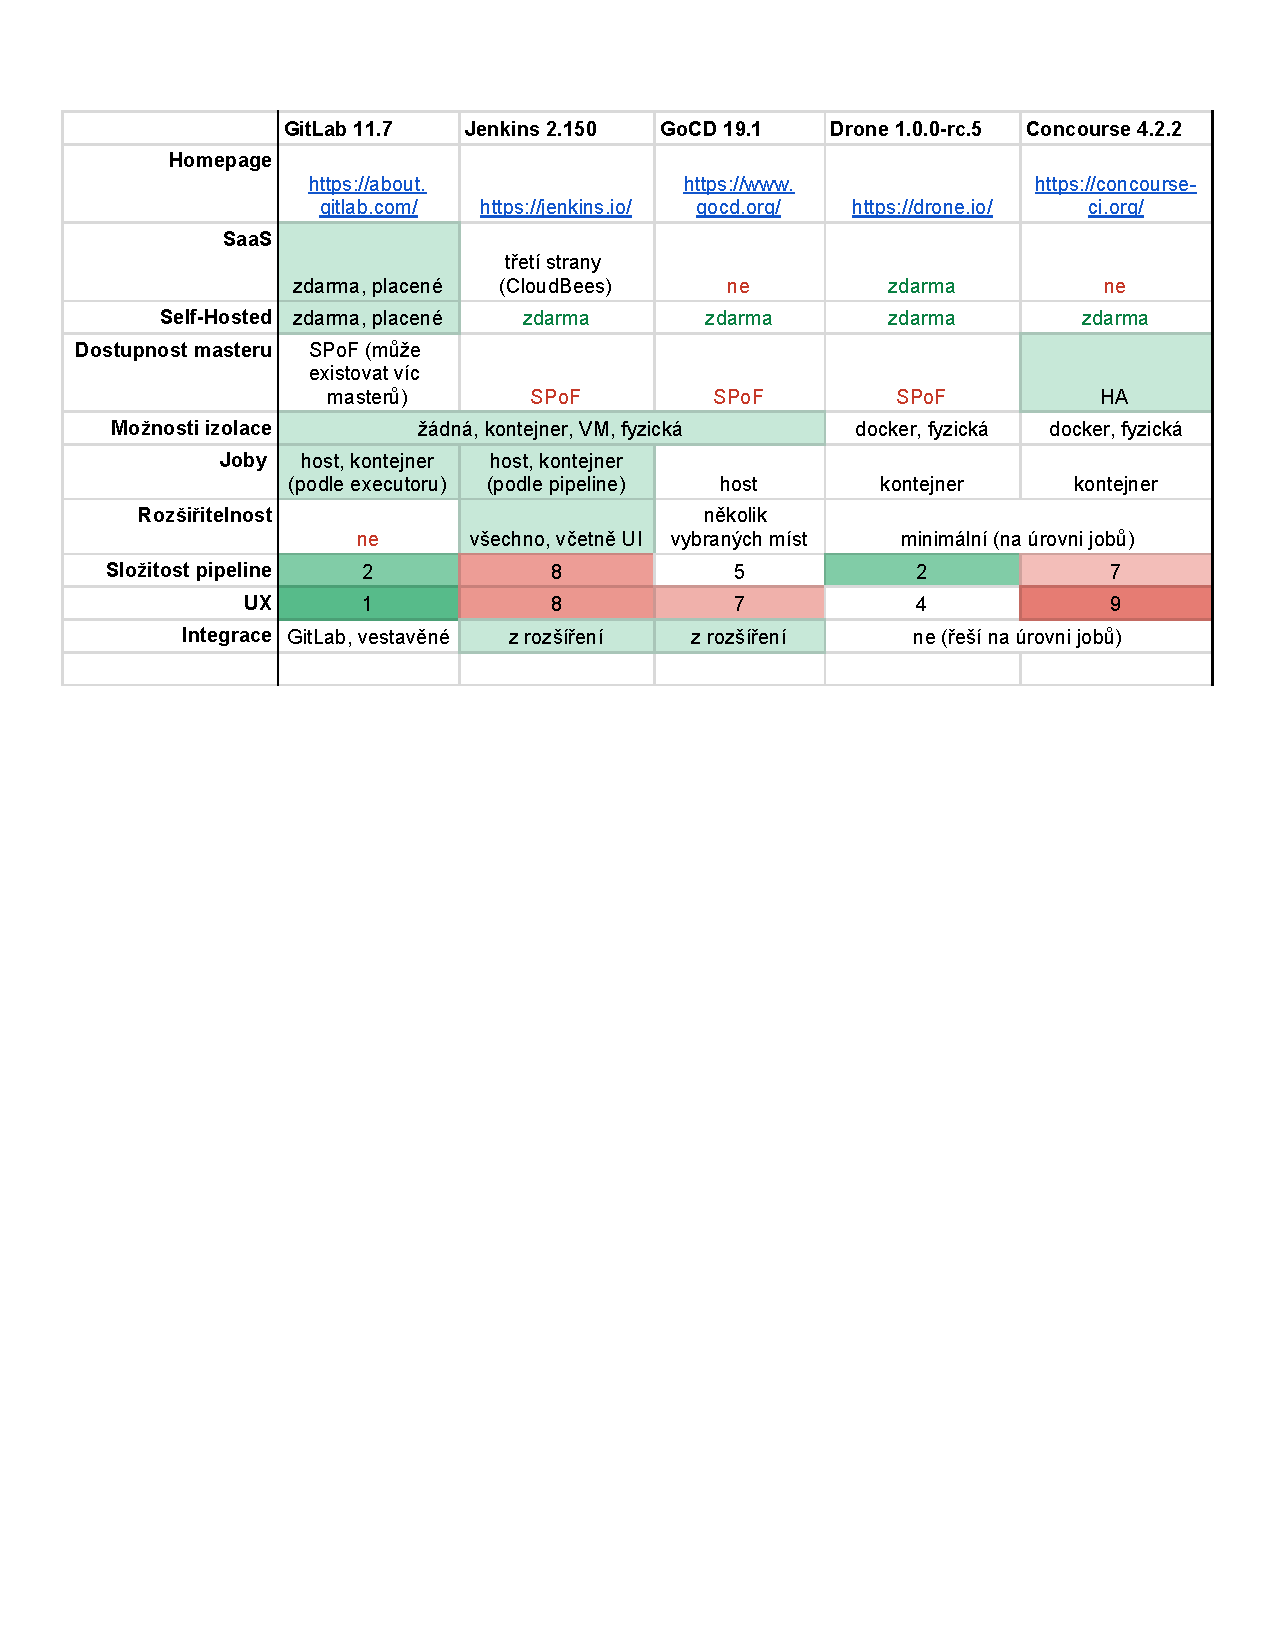
\includegraphics[page=1,width=1.4\textwidth]{media/porovnani-crop.pdf}
        }
    \end{center}

    \afterpage{
        \begin{center}
            \makebox[\textwidth][c]{
                \includegraphics[page=2,width=1.4\textwidth]{media/porovnani-crop.pdf}
            }
        \end{center}
    }

    Tabulka na této dvojstraně vizualizuje silné a slabé stránky porovnávaných \CI nástrojů. Zeleně podbarvené buňky reprezentují nejlepší hodnoty.

    S výjimkou GitLab jsou všechna \CI buď proprietární \glstext{SaaS} nebo zdarma, open-source a self-hosted. GitLab má odlišnou strategii a prodává licence i pro self-hosted variantu (GitLab \glstext{EE}).

    Dostupnost kontrolních serverů ma suverénně nejlepší Concourse, který umožňuje provozovat více masterů. GitLab může mít zaregistrováno více masterů (runnerů), ale každý se stará o svoji skupinu pipeline. Dostupnost agentů není uvedena. U všech \CI jsou joby stavové a z principu není možné je replikovat.

    Dále jsou \CI klasifikované podle úrovně izolace. Všechny self-hosted řešení nabízí izolaci kontejnery (ať už je přímo zabudovaná, je k dispozici pomocí rozšíření, nebo ji lze implementovat na úrovni samotného jobu). Díky master+agent architektuře lze také dosáhnout fyzické izolace, kde různí agenti běží na odlišných serverech. U \CI která nejsou postavená čistně na kontejnerech lze dosáhnout i žádné izolace. GitLab, Jenkins a GoCD ještě umožňují vytvářet dynamicky \glstext{VM}. U \glstext{SaaS} řešení která staví na kontejnerech není úplně jasné, jakou izolaci nabízí. Dá se ale očekávat, že uživatelé/organizace budou na oddělené \glstext{VM}.

    V řádku \textit{Joby} jsou porovnány možnosti konfigurace. U možnosti \textit{host} běží všechny příkazy na jedné \glstext{VM} a typicky nelze opakovat jenom části pipeline, ale konfigurace bývá intuitivnější. Oproti tomu varianta \textit{kontejner} označuje \CI, která rozdělují pipeline na různé části, kde každá se spouští v předem vytvořeném Docker kontejneru.

    Složitost pipeline a \glstext{UX} jsou čistě subjektivní relativní hodnocení. Škála je od 1 do 9, kde 1 je nejlepší skóre.

    \subsection{Použití jednotlivých \CI}
        \begin{description}
            \item[GitLab] Skvělé \CI. Podporuje jen repozitáře na GitLab. Dobrá podpora \CD díky integraci s Kubernetes.
            \item[Jenkins] Nejobecnější \CI s nejhorším \glstext{UX}. Použil bych až jako poslední možnost, pokud narazím na limitace jiných \CI.
            \item[GoCD] Funkčně stejné nebo horší než Jenkins, má menší komunitu, není tak udržovaný. Má nevýznamně lepší \glstext{UX}.
            \item[Drone] Minimalistické \CI. Cena stejná jako u GitLab, za řádově míň funkcí. Využil bych pro cloud-ready organizace, které pracují výhradně s kontejnery a mají repozitáře jinde než na GitLab.
            \item[Concourse] Alternativa ke Drone, má výrazně složitější konfiguraci a horší \glstext{UX}. Největši výhoda Concourse je vynikající dostupnost kontrolní roviny a cena.
            \item[CircleCI] \glstext{SaaS} varianta Drone. Limitující faktor je cena. V rozhodování můžou hrát roli izolace a rychlost.
            \item[Travis CI] \glstext{SaaS} varianta \CI nezaloženého na kontejnerech.
            \item[Semaphore CI] Alternativa k Travis~CI s komplikovanější konfigurací, ale za lepší cenu.
            \item[GitHub Actions] Novinka, pravděpodobně bude používané jako doplněk k dalším \CI.
        \end{description}

